\chapter{Foundations}
\label{ch:foundations}

The phenomena to be analyzed in this thesis include all methods to structure
and to describe digital data. To experience these phenomena we must first
broaden our view to see where they can be found. For this reason, this chapter
will first introduce the disciplines that deal with data and the description of
digital documents. This introduction also includes definitions of some basic
concepts and notations. These foundations are both used during collection and
analysis in the proceeding chapters and they can be instances of phenomena in
their own right. For instance mathematical set theory is used to define other
methods of data structuring, but set theory alone can also be used for data
structuring. We cannot fully avoid this circularity as every description must
be formulated in some other description --- basically this is the core problem
of data description. Nevertheless we can show how different disciplines
approach and tackle the problem. The largest part of this chapter introduces 
mathematics (section~\ref{sec:mathematics}) and computer science
(section~\ref{sec:informatics}) because these make the traditional foundations
of data: mathematics has proved to be an effective tool to exactly describe
structures of any kind and computer science provides the most examples, as most
problems of practical data processing belong to its domain. The approach of
library and information science (section~\ref{sec:lis}) is different: it is
basically concerned with the organization and description of documents. While
more and more documents become digital, the discipline should more and more
deal with data. The impact of philosophy is more subtle: as outlined in
section~\ref{sec:philosophy} there is not much explicit philosophy of data, but
philosophical issues permeate all other disciplines and philosophy helps to
reveal blind spots of other points of views. Semiotics
(section~\ref{sec:semiotics}) is relevant to this thesis because it deals with
signs and language, which all meaningful data is an instance of.
Section~\ref{sec:patterntheory} finally introduces the fundamental concepts
of patterns and pattern languages.  Both can be combined to pattern theory,
which is more a practice or an art than a scientific discipline.

\section{Mathematics}
\label{sec:mathematics}

\begin{quotation}%
As far as the laws of mathematics refer to reality, they are not certain;\\
and as far as they are certain, they do not refer to reality.\\
\quotationsource\Person[Albert]{Einstein}
\end{quotation}

\noindent Mathematics has proved to be an effective tool to exactly describe
structures of any kind.  This section introduces mathematical foundations and
notations that are referred to throughout the following chapters. It begins
with mathematical logic (section~\ref{sec:logic}) and set theory (section
\ref{sec:settheory}). Both have been used as foundation of mathematics and to
describe data types in computer science (see section \ref{sec:datatypes}).
Other methods to express data in mathematical terms are based on graph theory
(section~\ref{sec:graphtheory}).  Mathematics provides powerful methods of
formal description and to deductively draw conclusions from given axioms. Yet
it cannot prove this basic assumptions but only detect
inconsistencies.\footnote{As shown by \textcite{Goedel1931} mathematics can
even prove that in a system of axioms that is complex enough there are
consistent statements which cannot be proven or disproven without additional
axioms.} Despite the exactness of mathematics, to make use of it we must
carefully look out for which connections we draw between abstract structures
and anything outside of the domain of pure mathematics.

\subsection{Logic}
\label{sec:logic}

Mathematical \term{logic} has its origin in philosophy which also studied the
principles of valid reasoning. In particular the logic of \person{Aristotle}
was influential until the mid-nineteenth century, when a mathematical analysis
of logic was introduced by \textcite{Boole1847,Boole1854}. Mathematical logic
replaced natural language with formal symbols to express truth values and logical
statements. Typical notations include:

\begin{itemize}
\item $\bot$ or $1$ for true and $\top$ or $0$ for false
\item $\lnot$ for negation
\item $\land$ and $\lor$ for logical conjunction and logical disjunction
\item $\to$ and $\leftrightarrow$ for logical implication and logical equivalence 
\item symbols such as $a, b, x, y$ for variables and individual
  constants, independent of the ontological status of their referents
\end{itemize}

\noindent Alternative visual notations of logic systems, as introduced by
\textcite{Euler1768} and \textcite{Venn1880}, are dealed with in
section~\ref{sec:diagrams}.  The basic rules how to combine and interpret
statements from these formal symbols can defined by \term{Boolean algebra}.
Figure~\ref{fig:truthtables} contains laws of Boolean algebra and resulting
truth tables for the basic operations, $\lnot$, $\land$, $\lor$, $\to$ and
$\leftrightarrow$. Law 5 to 8 could also be derived from 1 to 4 and in total
there are 16 binary boolean operations.  The laws of Boolean algebra can be
used for \Term{inference}, that is to derive new logical statements from given
logical statements by \term[decduction]{deductive reasoning}\footnote{See also
figure~\ref{fig:reasong} for methods of reasoning.} For instance one can proof
that $\lnot(x \land y) \Leftrightarrow \lnot x \lor \lnot y$ and $\lnot(x \lor
y) \Leftrightarrow \lnot x \land \lnot y$ which is known as
\person[Augustus]{De Morgan}'s law.  The logic of Boolean algebra is equivalent
to \Term{propositional logic} and to the algebra of sets (see
section~\ref{sec:settheory}) among other descriptions. In particular, digital
switching circuits can be described by Boolean algebra \cite{Shannon1938},
which is the base of all digital computer systems.

\begin{figure}
\centering
\begin{tabular}{|ll|}
\hline
1. commutativity & $x \land y \Leftrightarrow y \land x$ \\ 
  & $x \lor y = y \lor x$ \\
2. distributivity & 
   $x \land (y \lor z) \Leftrightarrow (x \land y) \lor (x \land z)$ \\
 & $x \lor (y \land z) \Leftrightarrow (x \lor y) \land (x \lor z)$ \\
3. annihilation & $x \land 0 \Leftrightarrow 0$ \\
  & $x \lor 1 \Leftrightarrow x$ \\
4. excluded middle & $x \land \lnot x \Leftrightarrow 0$ \\
  & $x \lor \lnot x \Leftrightarrow 1$ \\
5. idempotence   & $x \land x \Leftrightarrow x$ \\
  & $x \lor x \Leftrightarrow x$ \\
6. associativity & $x \lor (y \lor z) \Leftrightarrow (x \lor y) \lor z$ \\
  &  $x \land (y \land z) \Leftrightarrow (x \land y) \land z$ \\
7. absorption
  & $x \land (x \lor y) \Leftrightarrow x \lor (x \land y) \Leftrightarrow x$ \\
8. logical identity & $x \land 1 \Leftrightarrow x$ \\
  & $x \lor 0 \Leftrightarrow x$ \\
\hline
\end{tabular}

\begin{tabular}{|c|c|}
\hline
$x$ & $\lnot x$ \\
\hline
0 & 1 \\
1 & 0 \\
\hline
\end{tabular}
\begin{tabular}{|cc|cccc|}
\hline
$x$ & $y$ & $x \land y$ & $x \lor y$ &
$x \to y$ & $x \leftrightarrow y$ \\
\hline
0 & 0 & 0 & 0 & 1 & 1 \\
0 & 1 & 0 & 1 & 1 & 0 \\
1 & 0 & 0 & 1 & 0 & 0 \\
1 & 1 & 1 & 1 & 1 & 1 \\
\hline
\end{tabular}
\caption{Laws of Boolean algebra and resulting truth tables}
\label{fig:truthtables}
\end{figure}

Further formalization of logical statements is possible with \Term{predicate
logic}, which extends \term{propositional logic} with predicates and
quantification. A logical \Term{predicate} is an individual symbol that refers
to a general statement with zero or more empty spaces. Predicates are typically
written in functional syntax, for instance $f(\_,\_)$ denotes the binary
predicate $f$ and $g(a)$ denotes the unary predicate $g$ where the space is $a$
filled by variable $a$. The number of spaces is called the predicate's
\Term{arity}. Predicates are logical statements insofar as they have a truth
value for each combination of individual variables. For instance $g(a)$ with
predicate $g$ and variable $a$ is either true or false. The ontological status
of predicates, however, is irrelevant to predicate logic: for instance
predicated could refer to properties (e.g. $g(a)$ $\Leftrightarrow$ `$a$ is
blue'), concept types ($g(a)$ $\Leftrightarrow$ `$a$ is a book'), relations
($f(a,b)$ $\Leftrightarrow$ `$a$ is friend of $b$'), or attributes ($f(a,b)$
$\Leftrightarrow$ `$a$ has size $b$'). Normal predicate logic (also known as
\Term{first-order predicate logic}) has two fundamental kinds of
\term{quantification}: universal quantification ($\forall$) to state that a
logical statement is true for all possible values of variable, and existential
quantification ($\exists$) to state that there is at least one value of a
variable that makes a logical statement true. If predicates and/or quantifiers
can be replaced by variables, predicate logic is extended to \term{higher-order
logic}. Higher-order logic allows more complex statements about statements, but
it is hard to verify statements even in second-order logic.  A common and less
complicated extension of predicate logic is the introduction of an identity
predicate or identity relation, also referred to as equality. With the
\Term{equality relation} `$=$' one can define a \Term{uniqueness quantifier} to
denote that exactly one object exists. We write $\exists!x : \phi(x)$ to
denote that there is only one $x$ for which $\phi(x)$ is true. The equality
relation can also be used to state that a statement is true for a specific
number of distinct values.  Further extensions and modification of
\term{propositional logic} and \term{predicate logic} are possible by adding
and by modification of the basic laws of Boolean algebra. For instance one can
argue against the law of excluded middle (law 4 in
figure~\ref{fig:truthtables}) and introduce a third truth value in addition to
true and false to denote `unknown' or `irrelevant' (\term{ternary logic}).
Other so-called non-classical logic extensions include:

\begin{itemize}
 \item an interval of possible truth values (\Term{fuzzy logic})
 \item additional quantifiers to express modality of statements (\Term{modal logic})
 \item elimination of the law of excluded middle and double negation so 
   statements only have a truth value only if they can explicitly be inferred 
   (\Term{intuitionistic logic})
 \item introduction of default values and exceptions (\Term{default logic})
 \item support of inconsistent statements (\Term{paraconsistent logic})
\end{itemize}

One example of modal logic relevant to data description is \Term{deontic
logic}, because this logic is concerned with obligation, permission, and norms
\cite{McNamara2010}. Deontic logic, however, includes several outstanding
philosophical problems: the basic problem, known as Joergensen's dilemma is
based on the relation of deontic values to logical truth values and
\cite{Jorgensen1937}: On the one hand norms cannot be true or false but only
fulfilled or violated, but on the other hand some norms seem to follow
logically from others. If one tries to formalize this implications, one may get
unexpected results such as the \term{Good Samaritan Paradox}: given that a
person is robbed and given that one should guard a person that is robbed, it
follows that a person should be robbed, because without robbery one cannot
guard anyone. 

The choice of a specific logic system and how it suits the domain to be
described is a philosophical question (see section~\ref{sec:philosophy}).  We
mostly assume classical logic, but on a closer look methods to structure and
describe data include non-classical elements, such as the introduction of
\term{NULL} values (\term{ternary logic}) and default values (\term{default
logic}), combined with annotations (\term{higher-order logic}). On the other
hand, data description should be easy to compute, so even \term{first-order
predicate logic} can be too complex --- there is no automatic method to decide
whether a general set of statements can be true (the problem is equivalent to
the problem of \Term{decidability} or \term{computability} described in
section~\ref{sec:informatics}). For this reason, subsets of \term{predicate
logic} called \Term{description logic} are preferred, especially for
\term{knowledge representation} \cite{Baader2010}. In description logic, only
specific kinds of statements are allowed with up to three variables. There are
unary predicates ($A, B, C\ldots$) to describe concept types, binary predicates
($R, S\ldots$) to describe relationships (also called `roles`), and a set of
possible methods to combine statements from these predicates. The statements in
description logic are typically divided into statements about concepts and
roles (\Term{TBox}) and statements that make use concept and role predicates
with concrete variables (\Term{ABox}).  A TBox together with an ABox are also
called a \term{knowledge base}.  Table~\ref{tab:dlogic} summarizes the
statement types of $\mathcal{ALC}$. This \Term{Attributive Concept Language
with Complements} is used as base of other description logics, some of which go
beyond predicate logic.\footnote{See \url{http://www.cs.man.ac.uk/~ezolin/dl/}
for an overview of description logic variants and their computable complexity.}
%For instance OWL~Lite = $\mathcal{SHIF(D)}$, OWL~DL = $\mathcal{SHOIN(D)}$
%etc. but \acro{ORM} cannot be fully expressed in \acro{DL} (Halpin2008, p.
%870).
%
To express and exchange logic statements in data there are some standards such
as \term{ISO Common Logic} \cite{ISO24707:2007}, \term{conceptual graphs}
\cite{Sowa1992,Sowa2000}, and controlled natural language \cite{Fuchs1999}.

\begin{table}
\centering
\begin{tabular}{|clll|}
\hline
& \textbf{description logic} & \textbf{notation} & \textbf{predicate logic} \\
\hline
TBox
& concepts                & $A, B, C\ldots$  & $A(x), B(x), C(x)\ldots$ (unary predicates) \\
& roles                   & $R, Q\ldots$     & $R(x,y), Q(x,y)\ldots$   (binary predicates) \\
& top concept             & $\top$           & $\forall x: \top(x)$ (predicate hold for all $x$) \\
& bottom concept          & $\bot$           & $\lnot \exists x: \bot(x)$ (predicate holds for no $x$) \\
& concept complement      & $\lnot C$        & $\lnot C(x)$ \\
& concept intersection    & $A\sqcap B$      & $A(x) \lor B(x)$  \\
& concept union           & $A\sqcup B$      & $A(x) \lor B(x)$ \\
& concept hierarchy       & $A\sqsubseteq B$ & $A(x) \to B(x)$ \\
& universal restriction   & $\forall R.C$ & $\forall y: R(x,y) \to C(x) $ \\
& existencial restriction & $\exists R.C$ & $\exists y: R(x,y) \to C(x) $ \\
\hline
ABox
& concept assertion       & $a:C$     & $C(a)$ \\
& role assertion          & $(a,b):R$ & $R(a,b)$ \\
\hline
\end{tabular}
\caption{Allowed types of logical statements in description logic $\mathcal{ALC}$}
\label{tab:dlogic}
\end{table}


\subsection{Set theory}
\label{sec:settheory}

Sets and properties occur in data description at least everywhere you deal with
multiple objects (see the `collections and types` paradigm in section
\ref{sec:collectionstopic}).  We hereby define `naive' set theory and notation
in natural language.  A deeper introduction and axiomatic definition that avoid
some paradoxes can be found by \textcite{Jech2003}.  In short, a \Term{set} is
a defined collection of objects. The objects in a set are called its
\Term[element!of a set]{elements} or \Term[member!of a set]{members}.  We write
$a \in A$ to denote that $a$ is \emph{a member of} the set $A$ or
\emph{contained in} the set $A$ and $a \notin A$ to denote that $a$ is not a
member of $A$. A set that contains no elements is called the \Term{empty set} and
denoted by $\set{}$ or $\emptyset$. The number of members in a set $A$ is
called its \Term{cardinality} and denoted by $|A|$. The cardinality of the set
of natural numbers $\mathbb{N}$ is denoted $|\mathbb{N}| = \aleph_0$.  Sets
with cardinality $\aleph_0$ are called \Term{countable infinite} in contrast to
a \Term{countable finite} set with finite number of elements.  The cardinality
of the continuum (the set of real numbers) is denoted
$|\mathbb{R}|=\mathfrak{c}$ which is strictly greater than $\aleph_0$.  If
every member of a set $A$ is also member of a set $B$ we call $A$ a
\Term{subset} of $B$ and write $A \subset B$. Reciprocally if every member of
$B$ is also member of $A$ then $B$ is a \Term{superset} of $A$ or
\Term[inclusion!of sets]{included} in $A$ and we write $B \supset A$. To denote
that $A$ is not a subset of $B$ we write $A \not\subset B$ and $B \not\supset
A$. If for two sets $A$ and $B$ both $A \subset B$ and $A \supset B$ then the
sets contain the same members and are called \Term[equality!of sets]{equal},
written as $A = B$. If $A$ and $B$ are not equal we write $A \neq B$. If $A$ is
a subset of $B$, but not equal to $B$, then $A$ is also called
\Term[proper!subset]{proper subset} of $B$ and we write $A \supsetneq B$ and $B
\subsetneq A$. A \Term[partition!of a set]{partition} of a set $A$ is a set of
subsets of $A$ such that every member of $A$ is exactly in one of the subsets
and none of the subsets is the empty set. Furthermore we define the following
operations on sets:

\begin{itemize}
 \item $A \cup B$ is the \Term[union!of sets]{union} of two sets $A$ and $B$, 
 which is the set of all objects that are members of one or both of the two sets.

 \item $A \cap B$ is the \Term[intersection!of sets]{intersection} of two sets 
 $A$ and $B$, which is the set of all objects that are members of both sets.

 \item $B \setminus A$ is the \Term[complement!of a set]{complement} of one set
 $A$ relative to another set $B$, which is the set of all objects that are not 
 members of $A$ but members of $B$.

 \item $\mathcal{P}$ is the \Term{power set} of a set $A$, which is the set of 
 all of its subsets. The set of all subsets with a given cardinality $n$
 is written as $\mathcal{P}_{n}(S)$.
\end{itemize}

To define particular sets, there are two methods. First, one can provide a
\Term[property!of set members|see{membership function}]{property} that all
members of the set must satisfy.  In set-builder notation we write
$\set[x]{\phi(x)}$ to denote the set of all elements that satisfy the property
$\phi$ and $\phi$ is also called the sets \Term{membership function}. For
instance the set of all prime numbers could be written as $\set[x]{x~\textrm{is
a prime}}$. With membership functions we can give more formal definitions of
operations on sets, for instance $A \cup B = \set[x]{x \in A \land x \in B}$.
Properties and sets can be used interchangeably: each property
defines a set and each set $A$ defines a property `being member of set $A$'.
Using properties to define sets, however, requires to somehow refer to a
collection of all possible members, which may or may not satisfy a property.
This collection is called the \Term{universal set} $\mathcal{U}$ or a
\Term{universe} if it is limited to some specific objects.  The second method
to specify a set is to write down a list of its elements in curly brackets. For
instance $\set{\times, \triangle, \heartsuit }$ can denote the set of a cross
symbol, a triangle symbol, and a heart symbol. Note that neither the order of
listed members nor any repetition of the same member is relevant --- the same
set could also be written as $\set{ \triangle, \heartsuit, \times, \triangle
}$. The identification of `same' elements is out of the scope of set theory
(unless elements are restricted to sets themselves). For instance the sets
$\set{ +, \blacktriangle, \texttt{<3} }$ and $\set{ \times, \triangle,
\heartsuit }$ both contains a cross symbol, a triangle symbol, and a heart
symbol. Whether both sets are equal depends on whether visual differences
between the symbols in both sets matter or not. Using properties such as
$\set{x|x~\textrm{looks like a heart symbol}}$ neither solves the \term{symbol
grounding problem}: arbitrary properties based on a general \term{universal
set} lead to paradoxes such  the impossible set $R = \set{ X | X \notin X }$
(\term{Russell's paradox}). This set is defined to contain all sets that do not
contain themselves, so $R$ must contain itself if it does not contain itself,
which is a contradiction. 

To avoid such paradoxes of naive set theory there are several strategies.
Zermelo-Fraenkel set theory with the axiom of choice assigns each set a
\Term[rank!of a set]{rank}, that is the smallest ordinal number greater than
the ranks of its members. There is no universal set but only the set
$\mathcal{V}_\alpha$ of all sets with rank $\alpha$. The full cumulative
hierarchy, starting with $\mathcal{V}_0 = \emptyset$, is called \Term{von
Neumann universe}. Another strategy adds \Term[class!in set theory]{classes}
or \Term[category]{categories} as distinct objects to sets. A class is defined
in the same way as a set, but it can only have sets as members. For every
property $\phi$ one can define the class $\Phi$ of all sets with property
$\phi$. Every set is also a class, but some \Term[proper!class]{proper
classes}, such as the class of all sets, and the paradoxical class $R$ cannot
be described as sets but only as classes. Classes and categories as
abstractions of sets and other mathematical objects are also studied in
\term{category theory}.

%\TODO{Basics of category theory and/or finite model theory may also be useful,
%because related to type theory, but I probably better skip them because of
%complexity. Maybe some aspects can be included in the section on sets or the
%section on tuples and relations, at least the term \Term{isomorphism}.}

% remark: We record that for defining a set one either needs to list its 
% distinct members or one needs to define a property.

% remark: hidden assumptions: data and referents are sets (but they mayb be not!)

% \TODO{Fuzzy sets may briefly be described here, if needed later.}

% Fuzzy sets are sets whose elements have a \Term{grade} of membership. Fuzzy
% sets have been introduced by Lotfi A. Zadeh (1965) as an extension of the
% classical notion of set...

\subsection{Tuples and relations}
\label{sec:relations}

Tuples and relation are mathematical constructs that appear at many places in
data description. They can best be defined based on set theory. A \Term{tuple}
is a finite ordered list, also known as sequence. A tuple with $n$ elements is
called an \Term{$n$-tuple}. The 2-tuple is also called \Term{ordered pair}. We
use angle brackets and write $\tuple{x_1 \ldots x_n}$ to denote the $n$-tuple
of $x_1$ to $x_n$. Similar to sets, tuples have members, but the order of
elements in a tuple is relevant ($\tuple{a,b} \neq \tuple{b,a}$). The same
element can also occur multiple times in a tuple ($\tuple{a,a} \neq \tuple{a}$ but
$\set{a,a} = \set{a}$).  Tuples are useful for further definitions of objects
with distinct members, for instance an $n$-ary \term{predicate} could be
defined as $n$-tuple. One applications of tuples is the definition of
mathematical relations.

A \Term{relation} is a set of similar tuples. More precisely, an $n$-ary
relation is a set of $n$-tuples $\tuple{x_1,x_2,\ldots x_n}$ and a set $n$ of
sets $X_1\ldots X_n$ where every element $x_i$ is member of some specific set
$X_i$. For each sequence of sets, there is a total relation, called the
\Term[product!of sets]{cartesian product}. Every $n$-ary relation is a subset
of a cartesian product, which is defined as: \[ X_1 \times X_2 \times \cdots
\times X_n = \set[\tuple{x_1,x_2\ldots x_n}]{x_i \in X_i, i=1\ldots n} \]

\index{recursive relation|see{digraph}}%
\index{relation!recursive|see{digraph}}%
%
A \Term{binary relation} $r$ between two sets $A$ and $B$ is some set of
ordered pairs $\tuple{a,b}$, where $a$ is element of $A$ and $b$ is element of
$B$. In this case, $A$ is called the \Term{domain} of $r$ and $B$ is the
\Term{codomain} of $r$, and we write $r: A \rel B$ (not to be confused with the
logical implication arrow $\to$).  The set of all such ordered pairs is the
cartesian product $A \times B = \set[\tuple{a,b}]{a \in A \wedge b \in B}$. The
sets of a relation do not necessarily have to be disjoint. For instance a
binary relation $r$ over a set $A$ is $r \subseteq A \times A$.  Binary
relations over sets are also studied in graph theory as these relations are
isomorph to \term{digraph}s (see section~\ref{sec:graphtheory}). In data
structures these relations are called \term{recursive}. Obviously one can turn
any binary relation over two sets $A$ and $B$ into a relation over one set $C$
with $C = A \cup B$.

Binary relations can be classified according to which kind of tuples they
contain. Table~\ref{tab:binaryrelprops} lists the most important types for a
binary relation $z: X \rel Y$. Part of the terminology was originally coined by
the Bourbaki group \cite{Bourbaki1970}. For functional relations the notation
$r(x)$ denotes the element from $r$'s codomain where $\tuple{x,r(x)}$ is in
$r$.  The \Term{domain of definition} and \Term{range} refer to the subset of
\term{term} and \term{codomain} that actually take part in the relation, but
the usage of this terms is not coherent and `domain' implicitly refers to the
domain of definition.  Figure \ref{fig:binaryrelations} illustrates the basic
terms and types with several binary relations over two out of four sets
$A=\set{a_1,a_2,a_3}$, $B=\set{b_1,b_2,b_3}$, $C=\set{c_1,c_2,c_3}$,
$D=\set{d_1,d_2,d_3}$ and its subsets $A'$, $B'$, and $D'$.  

\begin{table}
\centering
\begin{tabular}{|rl|}
\hline
\Term{injective} (left-unique)  
  & $\forall \tuple{x_1,y_1},\tuple{x_2,y_2} \in r: (y_1 = y_2) \rightarrow (x_1 = x_2)$ \\
\hline
\Term{functional} (right-unique) 
  & $\forall \tuple{x_1,y_1},\tuple{x_2,y_2} \in r: (x_1 = x_2) \rightarrow (y_1 = y_2)$ \\
\hline
\Term{one-to-one}
  & $\forall \tuple{x_1,y_1},\tuple{x_2,y_2} \in r: (y_1 = y_2) \leftrightarrow (x_1 = x_2)$ \\
\hline
(left-)\Term{total}
  & $\forall x \in X\, \exists y \in Y : \tuple{x,y} \in z$ \\
\hline
\Term{surjective} (right-total) 
  & $\forall y \in Y\, \exists x \in X : \tuple{x,y} \in z$ \\
\hline
\Term{function} or \Term{map}
  & $\forall x \in X\, \exists! y \in Y : \tuple{x,y} \in z$ \\
\hline
\Term{bijective} 
  & $\forall x \in X\, \exists! y \in Y : \tuple{x,y} \in z$ and \\
  & $\forall y \in Y\, \exists! x \in X : \tuple{x,y} \in z$ \\
\hline
\Term{correspondence}
  & $\forall x \in X\, \exists y \in Y : \tuple{x,y} \in z$ (total) and \\
  & $\forall y \in Y\, \exists x \in X : \tuple{x,y} \in z$ (surjective) \\
\hline
\end{tabular}
\caption{Types of binary relations}
\label{tab:binaryrelprops}
\end{table}

A bijective relation is also injective and surjective and a one-to-one
correspondence.  The extension of this concept in \term{category theory} is
called \term{isomorphism}, while structures that can be transformed injectively
or surjectively are called monomorphism or epimorphism, respectively. Binary
relations can also be combined to create new relations. The relation 
$g \circ f$ is defined as the set 
$\set[\tuple{x,z}]{\exists y: \tuple{x,y} \in f \wedge \tuple{y,z} \in g}$ (see 
figure \ref{fig:binaryrelations} for an example). 


\begin{figure}
\centering
\begin{tikzpicture}[orm,label distance=0mm]
  \begin{scope}
    \node[align=center,anchor=north,label=below:domain of $r$] (A)
      at (0,-2) {$A$};
    \draw[thick] (0,0) ellipse (1 and 1.7);
    \draw[thick,dotted] (0,0.3) ellipse (0.75 and 1);
    \node[gnode,label=below:$a_1$] (a1) at (0,0.8) {};
    \node[gnode,label=below:$a_2$] (a2) at (0,0) {};
    \node[gnode,label=below:$a_3$] (a3) at (0,-1) {};
    \draw[dotted] (0,1.4) -- (0,2) node[align=center,anchor=south]
      {$A'$ domain of\\definition of $r$};
  \end{scope}

  \begin{scope}[xshift=3cm]
    \node[align=center,anchor=north,label=below:codomain of $r$]
      (B) at (0,-2) {$B$};
    \draw[thick] (0,0) ellipse (1 and 1.7);
    \draw[thick,dotted] (0,0.3) ellipse (0.75 and 1);
    \node[gnode,label=below:$b_1$] (b1) at (0,0.8) {};
    \node[gnode,label=below:$b_2$] (b2) at (0,0) {};
    \node[gnode,label=below:$b_3$] (b3) at (0,-1) {};
    \draw[dotted] (0,1.4) -- (0,2) node[align=center,anchor=south,
      label=above:range of $r$] (B') {$B'$};
  \end{scope}

  \draw[garc] (a1) edge (b1) (a2) edge (b2) (a2) edge (b1);

  \begin{scope}[xshift=6cm,yshift=2mm]
    \node (C) at (0,1.8) {$C$};
    \draw[thick] (0,-.2) ellipse (1 and 1.55);
    \node[gnode,label=below:$c_2$] (c1) at (0,0.8) {};
    \node[gnode,label=below:$c_3$] (c2) at (0,-0.1) {};
    \node[gnode,label=below:$c_4$] (c3) at (0,-1) {};
  \end{scope}

  \draw[garc] (b1) edge (c1) (b2) edge (c2);

  \begin{scope}[xshift=9cm]
    \node[align=center,anchor=north] (D) at (0,-2) {$D$};
    \draw[thick] (0,0) ellipse (1 and 1.7);
    \draw[thick,dotted] (0,0.3) ellipse (0.75 and 1);
    \node[gnode,label=below:$d_1$] (d1) at (0,0.8) {};
    \node[gnode,label=below:$d_2$] (d2) at (0,0) {};
    \node[gnode,label=below:$d_3$] (d3) at (0,-1) {};
    \draw[dotted] (0,1.4) -- (0,2) node[align=center,anchor=south,
      label=above:range of $g$] (D') {$D'$};
  \end{scope}

  \draw[garc] (c3) edge (d2) (c1) edge (d1) (c2) edge (d2);

  \draw[thin,->] (A) edge node[above] {$r$} (B);
  \draw[thin,left hook->,in=180,out=-10] (B')
    edge node[above,pos=0.7] {$f$} (C);
  \draw[thin,->,out=0,in=-170] (C) edge 
    node[above,pos=0.3] {$g$} (D');
  \draw[thin,->,out=+10,in=170] (B')
    edge node[above] {$g \circ f$} 
         %node [below,pos=0.5,sloped,inner sep=2pt] {$\sim$} 
		 (D');
\end{tikzpicture}

\begin{tabular}{rccl}
& & & \\
relation & domain & codomain & type of relation \\
\hline
$r$	       & $A'$  & $B$  & left-total \\
	       & $A$   & $B'$ & right-total (or surjective or onto) \\
	       & $A'$  & $B'$ & correspondence (left- and right-total) \\
$f$        & $B'$  & $C$  & injective and partial function \\
	       & $C$   & $D$  & (total) function \\ 
$g$        & $C$   & $D'$ & surjective and function \\
$g\circ f$ & $B'$  & $D'$ & bijective \\
	       & $B$   & $D$  & one-to-one \\
\end{tabular}
\caption{Terms and types of binary relations}
\label{fig:binaryrelations}
\end{figure}

% TODO: need to explain?!:
% \textit{order} (\textit{transitive order}, \Term{total order}, %t
% \textit{partial order} \Term{strict order} \ldots)

\subsection{Graph theory}
\label{sec:graphtheory}

Formal graphs as method of description were introduced in the late 19th century
by \textcite{Cayley1857} and \textcite{Sylvester1878} for chemical structures.
Among other applications, graphs can be used to model binary relations over a
set of objects. Most of the following definitions can be found in any
introduction to graph theory but terminology differs among authors in slight
details.

A \Term{graph} is a pair $\tuple{V,E}$ where $V$ is a finite set of
\textit{nodes} \index{node!of a graph} (or \textit{vertices})
\index{vertex|see{node}} and $E$ is a finite set of \textit{edges}\index{edge}.
Unless otherwise indicated the graph is a \Term{simple graph}, that means edges 
are 2-sets without orientation and cannot connect a node with itself:
$E \subseteq \mathcal{P}_{2}(V)$ Two nodes $u,v$ are \Term{adjacent} if
$\set{u,v} \in V$. The \Term{degree} of a node $v$ is the number of adjacent
nodes $\set[u]{\set{u,v} \in V}$. A \Term{path} is a sequence of two or more
nodes $v_1,\ldots v_n$ such that $v_i$ and $v_{i+1}$ are adjacent for 
$1 \le i < n$. Unless otherwise noted a path uses every edge at most once. 
A \Term{cycle} is a path with $v_1=v_n$. If there is a path between two nodes
$u$ and $v$, they are \Term{connected} and their \Term{distance} is the length
of their shortest connecting path. A graph is said to be connected if every pair
of nodes in the graph are connected. Unless otherwise noted a graph is
assumed to be connected. A \Term{planar graph} can be drawn on a plane without
intersecting edges. A graph is \Term[bipartite graph]{bipartite} if its nodes
can be partitioned into two sets such that no nodes of the same set are
adjacent. Unless mentioned otherwise we will use the term \term{bipartite
graph} more specific for a \Term{fixed bipartite graph} $\tuple{V_1,V_2,E}$ with
specific node partition -- which is isomorph to a binary relation (see 
example~\ref{ex:hypergraph}).

\begin{figure}
\centering
\begin{tikzpicture}
  \begin{scope}[every node/.style={gnode}]
    \node (A) at (0,0) {}; \node (B) at (1,0) {}; \node (C) at (2,0) {};
    \path[garc] (A) edge (B) (B) edge (C);
  \end{scope}
  \node at (1,-.5) {\ormtext\textbf{a)} sequence graph};
  \begin{scope}[every node/.style={gnode},xshift=3cm]
    \node (A) at (0.5,1) {};
    \node (B) at (1.5,1) {};
    \node (C) at (0.0,0) {};
    \node (D) at (1.0,0) {};
    \node (E) at (2.0,0) {};
    \node (F) at (2.5,1) {};
    \path[garc] (A) edge (B) (C) edge (A) (C) edge (D) 
                (D) edge (E) (E) edge (B) (D) edge (B) (E) edge (F);
  \end{scope}
  \node at (4.25,-.5) {\ormtext\textbf{b)} acyclic digraph (DAG)};
  \begin{scope}[every node/.style={gnode},xshift=6.5cm,yshift=-1cm]
    \node (A) at (0.5,3) {};
    \node (B) at (1.5,3) {};
    \node (C) at (2.0,2) {};
    \node (D) at (1.5,1) {};
    \node (E) at (0.5,1) {};
    \node (F) at (0.0,2) {};
    \path[garc] (A) edge (B) (B) edge (C) (C) edge (D) 
                (D) edge (E) (E) edge (F) (F) edge (A);   
  \end{scope}
  \node at (7.5,-.5) {\ormtext\textbf{c)} cycle graph};
  \begin{scope}[xshift=10.5cm,yshift=1cm]
    \matrix[row sep=.8cm,column sep=.8cm,every node/.style={gnode}] {
      \node (A) {}; & \node (B) {}; & \node (C) {}; \\
      \node (D) {}; & \node (E) {}; & \node (F) {}; \\
      \node (G) {}; & \node (H) {}; & \node (I) {}; \\
    };
    \path[garc] (A) edge (B) (B) edge (C) (D) edge (E)
                (E) edge (F) (G) edge (H) (H) edge(I);
    \path[garc] (A) edge (D) (B) edge (E) (C) edge (F)
                (D) edge (G) (E) edge (H) (F) edge (I);   
  \end{scope}
  \node at (10.5,-.5) {\ormtext\textbf{d)} grid graph};
\end{tikzpicture}
\caption{Some digraph types exemplified}
\label{fig:digraphtypes}
\end{figure}

A \Term{directed graph} or \Term{digraph} is a graph whose edges (also called
\textit{arcs}) are ordered pairs: $E \subseteq V \times V$. An arc $\tuple{u,v}$
is said to direct, link, or point from $u$ to $v$; unless otherwise indicated a
\Term{loop}, that is an arc that pairs a node to itself ($u=v$), is not allowed.
An arc $\tuple{u,v}$ is \Term{symmetric} if its reverse link $\tuple{v,u}$ is
also present. A simple graph can be modeled by a digraph that only holds
symmetric links. In a digraph we must distinguish the number of edges pointing
to a node as \Term{indegree} and the number of edges pointing from a node as
\Term{outdegree}. A (directed) \textit{path}\index{path} is a non-empty sequence
of nodes, one pointing to the next without use a link twice. A node $u$ is
\Term{reachable} from another node $v$ if there is a directed path from $v$ to
$u$. A path that starts and ends in the same node is a \textit{\term{cycle}}.
If a node $u$ can be reached from $v$ on two disjoint paths, the union of
both paths is called a \Term{diamond}. Adding all reverse links to a
diamond results in a cycle. A digraph is \Term{strongly connected} if every node
is reachable from every other node and \Term{weakly connected} if adding all
missing symmetric links would result in a strongly connected digraph. Unless
otherwise noted a digraph is assumed to be weakly connected.

Some types of directed graphs deserve special treatment: A \Term{sequence graph} 
(figure~\ref{fig:digraphtypes}~{\ormbf a}) is a strongly connected digraph in
which only one one node has indegree 0 and all other nodes have indegree 1.
A (directed) \Term{cycle graph} ({\ormbf c}) is a digraph that consists of a
single cycle. A \Term[directed acyclic graph (DAG)]{directed acyclic graph}
(DAG) or \Term{acyclic digraph} ({\ormbf b}) is a directed graph containing no
cycles. \index{acyclic digraph graph|see{directed acyclic graph (DAG)}}
The edges of a (directed) \Term{grid graph} ({\ormbf d}) are defined by a
$n$-tuple $\tuple{s_1,\ldots,s_d}$ where $d$ is the \Term[dimension!of a grid
graph]{dimension} of the graph and $s_i \in \mathbb{N}^+$ are its
\Term[size!of a grid graph]{sizes}.

% define: \mathbb{N}^+

% The nodes of a grid graph are bijectively mapped to the set of
% \Term[coordinate!in a grid graph]{coordinates} which is
% $C=\set[\tuple{p_1,\ldots,p_n}]{0 \le p_i < s_i}$. For every combination of
% coordinates $c_1,c_2 \in C$ there is a directed edge from the lower coordinate
% to the higher coordinate if and only if their distance is one.

\begin{example}
\centering
\begin{tikzpicture}[orm,label distance=1mm]
  \begin{scope}[every node/.style={gnode}]
   \node[label=left:$a_1$] (A) at (0,2) {};
   \node[label=right:$a_2$] (B) at (1,2) {};
   \node[label=left:$a_3$] (C) at (0,1) {};
   \node[label=right:$a_4$] (D) at (1,1) {};
   \node[label=left:$a_5$] (E) at (0,0) {};
   \node[label=right:$a_6$] (F) at (1,0) {};
  \end{scope}
   \draw[gedge] (C) edge (0.7,1.4) (0.7,1.4) edge (B) (D) edge (0.7,1.4);
   \draw[gedge] (A)--+(0.4,0) node[anchor=south] {$b_1$};
   \node at (0.5,1.6) {$b_2$};
   \draw[gedge] (C) -- node[anchor=west] {$b_3$} (E);
  \node at (0.5,-1) {{\ormbf a)} hypergraph};
  \node at (2,1) {$\simeq$};

  \begin{scope}[xshift=3cm,every node/.style={gnode}]
   \node[label=left:$a_1$] (A) at (0,2.25) {};
   \node[label=left:$a_2$] (B) at (0,1.75) {};
   \node[label=left:$a_3$] (C) at (0,1.25) {};
   \node[label=left:$a_4$] (D) at (0,0.75) {};
   \node[label=left:$a_5$] (E) at (0,0.25) {};
   \node[label=left:$a_6$] (F) at (0,-.25) {};
   \node[label=right:$b_1$] (a) at (1.2,2.25) {};
   \node[label=right:$b_2$] (b) at (1.2,1.25) {};
   \node[label=right:$b_3$] (c) at (1.2,0.5)  {};
  \end{scope}
  \begin{scope}[xshift=3cm]
   \draw[garc] (A) edge (a) (B) edge (b) (C) edge (b) 
               (D) edge (b) (C) edge (c) (E) edge (c);
  \end{scope}
  \node at (3.75,-1) {{\ormbf b)} bipartite graph};

  \begin{scope}[xshift=5.5cm]
  \node[anchor=west] at (0,2.4)  {$A=\set{a_1,a_2,a_3,a_4,a_5,a_6}$};
  \node[anchor=west] at (0,1.9)  {$B=\set{b_1,b_2,b_3}$};
  \node[anchor=west] at (.3,1.4) {$=\{\{a_1\},\{a_2,a_3,a_4\},\{a_3,a_5\}\}$};
  \node[anchor=west] at (0,0.9)  {$V=A \cup B$};
  \node[anchor=west] at (0,0.4)  {$E=\set[\tuple{v,e}]{e \in A, v \in e}$};
  \node[anchor=west,align=right] at (.3,-.3) 
   {$=\{\tuple{a_1,b_1},\tuple{a_2,b_2},\tuple{a_3,b_2},$\\
     $\tuple{a_4,b_2},\tuple{a_3,b_3},\tuple{a_5,b_3}\}$};
  \end{scope}
  \node at (7.5,-1) {{\ormbf c)} surjective relation (E)};
\end{tikzpicture}
\caption{A hypergraph and its (fixed) bipartite graph}
\label{ex:hypergraph}
\end{example}

The graph concept can be further extended: A \Term{multigraph} is a
graph in which multiple edges can exist between any two nodes. The maximum
number of edges linking two nodes is called the \Term{multiplicity} of the
multigraph. A multigraph can be defined two ways: Either the edges $E$ do not
form a set but a bag; in this case multiple edges are indistinguishable. Or the
two nodes that are connected by an edge are not their element but but there
is an additional function $\vartheta: V \rel E \times E$ that maps edges to
node-pairs. There can be simple and directed multigraphs. Unless defined
otherwise edges are not ordered.

In a \Term{hypergraph} an edge can connect any positive number of nodes. The
edges of a hypergraph are also called \Term{hyperedge}. There is an isomorphism
between hypergraphs and fixed bipartite graphs that have no unconnected nodes
in the second partition (example~\ref{ex:hypergraph} {\ormtext b}): Let
$H=\tuple{A,B}$ with $B \subseteq \mathcal{P}(A) \setminus \emptyset$ be a
hypergraph. You can then construct a directed bipartite graph $P=\tuple{V,E}$
as shown in example~\ref{ex:hypergraph}, or express the hypergraph as
surjective relation between two disjoint sets. By lifting the disjointness
constraint, one gets a \Term{generalized hypergraph} in which edges can also
connect other edges.  This neutralizes the distinction between nodes and edges
-- if the graph is also a multigraph, one can simply view nodes as empty edges.
It is easier to visualize generalized hypergraphs as directed acyclic graphs
(if edges can only contain edges of smaller rank) or as general directed
graphs. Nodes of the new graph correspond to edges in the hypergraph and edges
represent edge containment. This representation of a generalized hypergraph is
sometimes called \term{Levi graph}.

% http://wiki.github.com/tinkerpop/gremlin/modeling-hypergraphs

There are several forms of \Term{graph labeling}, that is the assignment of
labels, or other elements to edges, nodes, or both of a graph. We define a
\Term{property graph} as tuple $\tuple{V,E,P,\Phi}$ with $E$ being a
finite set of edges, $V$ being a finite set of nodes, $P$ being a finite set
of properties and $\Phi: G' \rel P$ with $G' \subseteq (V \cup E)$ a partial
function that maps edges and/or nodes to properties. For $\Phi: E \rel P$
(only edges have properties) the graph is a \Term{edge-property graph} and for
$\Phi: V \rel P$ (only nodes have properties) it is a \Term{node-property
graph}. This definition makes no assumption on the nature of nodes and thus
can be applied to all kinds of graphs (simple graphs, directed graphs,
multigraphs, hypergraphs). There is no assumption on properties: they can
be labels, types, weights, colors, identifiers, attributes, sets, tuples etc.
depending on the particular property graph type. A relevant instance is a
property graph where $(V \cup E)$ can be mapped via \term{bijection}
to $P$ so every node and edge can be identified uniquely by its property.

\begin{figure}
\centering
 \begin{tikzpicture}
  \begin{scope}[every node/.style={gnode}]
    \node at (0.5,2) (A) {};
    \node at (0,1) (B) {};
    \node at (1,1) (C) {};
    \node at (2,1) (D) {};
    \node at (0.5,0) (E) {};
    \node at (3,0.5) (F) {};
    \node at (3,1.5) (G) {};
    \path[gedge] (A) edge (C) (B) edge (C) (E) edge (C) (C) edge (D)
                 (C) edge (D) (D) edge (F) (D) edge (G);
  \end{scope}
  \node at (1.5,-.5) {\ormtext \textbf{a)} undirected tree};
  \begin{scope}[every node/.style={gnode},xshift=4cm]
    \node (A) at (1,2) {};
    \node (B) at (0.5,1) {};
    \node (C) at (1.5,1) {};
    \node (D) at (0,0) {};
    \node (E) at (1,0) {};
    \node (F) at (2,0) {};
    \path[garc](A) edge (B) (A) edge (C) (B) edge (D) (C) edge (E) (C) edge(F);
    \path[glink] (B) edge (C) (E) edge (F);
  \end{scope}
  \node at (5,-.5) {\ormtext \textbf{b)} ordered tree};
  \begin{scope}[every node/.style={gnode},xshift=7cm]
    \node at (0,2) (A) {};
    \node at (1,2) (B) {};
    \node at (2,2) (C) {};
    \node at (0.5,1) (D) {};
    \node at (1.5,1) (E) {};
    \node at (0,0) (F) {};
    \node at (1,0) (G) {};
    \node at (2,0) (H) {};
    \path[garc] (A) edge (B) (B) edge (E) (C) edge (E)
                (D) edge (F) (D) edge (G) (E) edge (G) (E) edge (H);
  \end{scope}
  \node at (8,-.5) {\ormtext \textbf{c)} polytree};
  \begin{scope}[every node/.style={gnode},xshift=10cm]
    \node at (0.5,2) (A) {};
    \node at (0,1) (B) {};
    \node at (1,1) (C) {};
    \node at (2,1) (D) {};
    \node at (0.5,0) (E) {};
    \node at (1.5,0) (F) {};
    \node at (1.5,2) (G) {};
    \path[garc] (A) edge (B) (A) edge (C) (E) edge (C) (E) edge (B) (C) edge (D)
                (C) edge (F) (A) edge (G);
  \end{scope}
  \node at (11,-.5) {\ormtext \textbf{d)} multitree};
\end{tikzpicture}
\caption{Tree types}
\label{fig:treetypes}
\end{figure}

\Term*{tree}
An \Term{undirected tree} (figure~\ref{fig:treetypes}~{\ormbf a}) is a
simple graph without cycles. Tree nodes with degree one are also called
\Term[leaf]{leafs}. An unconnected tree is called a \Term{forest}. By
selecting a single tree node as \Term[root!of a tree]{root}, one gets a 
\Term{rooted tree} ({\ormbf b} without the dashed lines). This
selection implies a direction on every edge. The direction is typically defined
pointing outwards from the root. Unless noted otherwise the term tree will be
used for such rooted trees. By reversing the direction on all edges, one gets
\Term{inverted tree}. The tree nodes that are directly connected from a
given node via one outgoing edge are its \term{child node} which are
\term{siblings} to each other. All nodes reachable from another are its
\Term[descendant]{descendants} which for a subtree. All nodes that can reach
another node are its \Term[anchestor]{ancestors} which form a sequence graph
starting from the root. An \Term{ordered tree} is a tree in which the
child nodes of each node are ordered. In (figure~\ref{fig:treetypes}~{\ormbf b})
ordering is indicated by dashed linkes pointing from one sibling to the next.
% TODO: see section XX on how to implement (orderd) trees
There are two special kinds of DAGs that are also called trees: A
\Term{polytree} ({\ormbf c}) is a directed acyclic graph containing no
undirected cycles and a \Term{multitree} ({\ormbf d}) is directed
acyclic graph without directed diamonds \cite{Furnas1994}. In a multitree the
descendants of any node form a tree and the ancestors of any node form an
inverted tree but there may be undirected diamonds. Every polytree is also a
multitree and every directed tree is also a polytree.


\section{Computer science}
\label{sec:informatics}

\begin{quotation}%
Any sufficiently advanced technology is indistinguishable from magic.
\\ \quotationsource \Person[Arthur C.]{Clarke}
\end{quotation}

\noindent
The following sections introduce three topics from computer science that 
are relevant to this thesis: \emph{formal languages} and computation are 
fundamental computer science concepts to reason about sets of data 
(section~\ref{sec:formallanguages}). \emph{Data types} are important to 
manage data structures in programming languages and in databases 
(section~\ref{sec:datatypes}). Finally, \emph{data modeling} tries to bridge 
the gap between  some reality and its description in form of data in some 
information system (section~\ref{sec:datamodeling}). First the discipline
should be put in context by a short overview.

In general, computer science deals with the theoretical and practical 
automatic processing of data or information. The first scientific computing 
organization was founded in 1947 with the \tacro{Association for Computing 
Machinery}{ACM}. Computer science as an independent academic field was 
established until the 1960s. The history of the discipline, which can be 
located somewhere between applied mathematics and engineering, is 
directly connected to the development and application of computer systems. 
The first computers as programmable, general purpose machines were created in 
the 1940s for military calculations.%
\footnote{The first computers include: Zuse Z3 (1941) and Z4 (1945) 
that were created for calculations in military aviation, as
well as other early German calculating machines from this time 
\cite[p. 202ff.]{Lange2006};
Collosus (1944) that helped to decipher encrypted messages by British 
codebreakers; Harvard Mark~I/ASCC (1944) and its successors that were 
used by the US Navy; ENIAC (1946) and EDVAC (1949) that were used by 
the US Army. Only the IBM SSEC (1948) also served non-military purposes 
until in 1949 three computers were completed at research institutions, partly
with commerical support: EDSAC in Cambridge, Manchester Mark~1 in Manchester,
and CSIRAC in Sydney.
% More limted systems to solve equations existed before:
% Only the limited Atanasoff-Berry-Computer (1942) had no military application.
% but it was limited to solve equations like other equation solvers
% e.g. Differential analysers (Bush etc.)
% Rockefeller Differential Analyzer (1942, invented 1931 by Vannevar Bush)
More about early computers can be found in the collection by
\textcite{Rojas2000}.}
Meanwhile, computers are used in almost any aspect of daily live with an
impact comparable to the industrial revolution or with the invention of 
the printing press. The economic weight of the so called information industry
is another factor that must be beard in mind when thinking about promises 
and motivations of (applied) computer science.

From the beginning of computer science, there has been a tendency to 
describe computers not only as tools for automatic data processing, but to 
attribute them with human terms like `intelligent', `thinking', `knowledge', 
`brain`, and `semantic'.\footnote{See for instance \textcite{Berkeley1949} 
and the whole terminology of artificial intelligence. Even the term `language'
is misleading because programming languages and other formal languages,
unlike human languages, are based on precise formalization but not on speech
and communication \cite{Naur1992}.} % TODO: pagenum of Naur 1992!
The comparision of automatic systems with brain power is also drawn, if 
computing is viewed as a natural phenomenon, with mental activity as
instances of information processing, similar to computer systems 
\cite{Denning2007}.

The traditional, rationalistic paradigm of computer science is contrasted
by constructivist views that stress the relativity of automatic systems
as social artifacts. For Turing Award winner\footnote{The Turing Award, 
annually awarded by the \acro{ACM} is the highest distinction in computer
science.} \Person[Peter]{Naur}, pioneer in \term{software engineering} who 
suggested the term \term{datalogy} in favour of computer science, programming
is not comparable to industrial production, but an act of theory building 
\cite{Naur1985}, and ``the core of programming is the programmer's developing
a certain kind of understanding of the matters of concern.'' \cite{Naur2007}.%
\footnote{See \textcite{Wyssusek2007} for a more detailed discussion of Naur's
position.} Despite the predominant practice in computer science, computing 
artifacts are neither objective description of reality \cite{Kent1978} nor
an optimal solution of a given problem. Instead ``we construct the problem 
as well as the solution'' \cite{Floyd1996} and must therefore take 
responsibility for the thus constructed reality \cite{Weizenbaum1976}.
Having said this, computer science provides powerful theories and tools
to describe and process data.

\subsection{Formal languages and computation}
\label{sec:formallanguages}
\index{language!formal languages}

The study of formal languages emerged independently during the 1950s in
linguistics and in computer science: \Person[Noam]{Chomsky} applied it to human
languages, and \Person[John]{Backus} to programming languages
\cite{Greibach1981}. The basic properties of formal grammars, languages, and
computation are explained by \textcite{Hopcroft1979}.  A \Term{formal language}
is a defined set of sequences of symbols. The symbols are also called the
\Term{alphabet} of the language, and the sequences are also called
\term[string]{strings} or \Term[word]{words}. Examples of formal languages
include: the set of words that can be build as sequences of the letters A to Z;
the set of roman numerals with symbols I,V,X,L,C,D,M; and the set of
genome sequences with adenine, cytosine, guanine, thymine as symbols.  A
formal language can be defined by either listing all of its words, if the
language is finite, or by specifying a membership property that all of its
words must satisfy. In computer science formal languages are studied in form of
their membership properties, as automata or formal grammars, which will both be
described in the following.

An \Term{automaton} is an mathematically defined method (a process or
algorithm) to compute whether a string belongs to a given formal language. The
automaton is said to \Term[decidability]{decide} whether a string belongs to
the language, if the method is guaranteed to halt with positive or negative
result after a finite amount of time. As shown first by \textcite{Turing1936}
and \textcite{Church1936}, there exist formal languages which are
\Term[decidability]{undecidable}: that means no automatic process can compute
whether a string belongs to the language or not: any algorithm at least for
some strings will not halt computation in finite time.\footnote{The proof
provided by \textcite{Turing1936} is known as `halting problem': in particular
the formal language of `all programs that will halt' is not decidable.} The
concept of decidability is based on the concept of \Term{computation}, which is
a core concept of the whole discipline of computer science. Crucial for the
concept of computation is the idea of a process where all steps are precisely
defined. There are several models of computation which can be grouped in
classes of equivalent computational power. A model of computation that belongs
to the most powerful class is said to be \Term{Turing-complete}, and it can be
used to compute all computable problems, as stated by the Church-Turing-thesis.
The terms `computable' and `decidable' can be used interchangeably, as all
functions with enumerable \term{domain} can be expressed as formal languages
with tuples as words.

A \Term{formal grammar} is a set of rules that describe how to form words of a
formal language. It consists of the alphabet of symbols $A$, one selected
\Term{starting symbol} $S\in A$, and a set of \Term{production rules}, each
rule of the form $\alpha \rightarrow \beta$, where $\alpha$ and $\beta$ are
sequences of symbols. The empty sequence $\epsilon$ can also be allowed, for
instance to express removal of a sequence  ($\alpha \rightarrow \epsilon$).  To
better analyze formal grammars, the alphabet is partitioned in two sets:
\Term{terminal symbols} may occur in words and \Term{non-terminal symbols}
occur only as variables, that are replaced by other sequences during the
production process.  Example~\ref{ex:romannum} shows a formal grammar that can
produce all roman numerals up to 4999, or the empty sequence. The grammar can
also be written in more concise form as regular expression.\footnote{% The
grammar has been adopted from a \term{regular expression} that was kindly
provided and explained by user `paxdiablo' at
\url{http://stackoverflow.com/questions/267399/\#267405}.} Regular expressions
and other methods to express formal grammars will be described in
section~\ref{sec:bnf}.

\begin{example}[h]
\begin{centering}
\begin{tabular}{ |l|p{0.7\linewidth}| }
\hline
starting symbol & $S$ \\
\hline
terminal symbols & I, V, X, L, C, D, M, $\epsilon$ \\
\hline
non-terminals &
$T$ for thousands, 
$H$ for hundreds,
$E$ for hundreds from $\epsilon$ to CCC,
$Z$ for tens,
$Y$ for tens from $\epsilon$ to XXX,
$U$ for units,
$O$ for units from $\epsilon$ to III
\\
\hline
production rules &
$S \rightarrow THEU $

$T \rightarrow \epsilon \ ,\  
 T \rightarrow \textrm{M} \ ,\  
 T \rightarrow \textrm{MM} \ ,\ 
 T \rightarrow \textrm{MMM} \ ,\ 
 T \rightarrow \textrm{MMMM}$

$H \rightarrow E \ ,\ 
 H \rightarrow \textrm{CM} \ ,\ 
 H \rightarrow \textrm{CD} \ ,\ 
 H \rightarrow \textrm{D}E $

$E \rightarrow \epsilon \ ,\ 
 E \rightarrow \textrm{C} \ ,\  
 E \rightarrow \textrm{CC} \ ,\  
 E \rightarrow \textrm{CCC}$

$Z \rightarrow Y \ ,\ 
 Z \rightarrow \textrm{XC} \ ,\
 Z \rightarrow \textrm{XL} \ ,\    
 Z \rightarrow \textrm{L}Y $

$Y \rightarrow \epsilon \ ,\ 
 Y \rightarrow \textrm{X} \ ,\  
 Y \rightarrow \textrm{XX} \ ,\  
 Y \rightarrow \textrm{XXX} $

$U \rightarrow O \ ,\  
 U \rightarrow \textrm{IX} \ ,\  
 U \rightarrow \textrm{IV} \ ,\  
 U \rightarrow \textrm{V}O$

$O \rightarrow \epsilon \ ,\ 
 O \rightarrow \textrm{I} \ ,\  
 O \rightarrow \textrm{II} \ ,\  
 O \rightarrow \textrm{III} $
\\
\hline
\end{tabular}
\end{centering}
%\\
The language could also be expressed by the 
following regular expression:\\
~\verb!^M{0,4}(CM|CD|D?C{0,3})(XC|XL|L?X{0,3})(IX|IV|V?I{0,3})!
\caption{Formal grammar of roman numerals up to 4999}
\label{ex:romannum}
\end{example}

Unrestricted formal grammars are Turing-complete, so any computable process can
also be encoded as a formal grammar. For instance \term[functional
programming]{Functional programming} languages like \term{Haskell} make use of
\term{rewriting system}s, as shown below. By putting restrictions on the
general form of production rules and/or on the process of replacing sequences
by applying rules, one can define subclasses of formal languages with less
complexity. The most known classification is the \Term{Chomsky hierarchy} with
the following languages:

\begin{itemize}
\item Type-0: \Tacro{recursively enumerable languages}{RE} include all 
 languages that can be defined by any formal grammar. Rules have the form
 $\alpha \rightarrow \beta$ where $\alpha$ and $\beta$ are unrestricted
 sequences of symbols.
\item Type-1: \Tacro{context-sensitive languages}{CSL} have production
 rules of the form $\alpha X\beta \rightarrow \alpha\gamma\beta$
 where $X$ is a non-terminal symbol; $\alpha$, $\beta$, $\gamma$ are
 sequences of symbols; and only $\alpha$ and $\beta$ can be empty.
 In addition, a rule of the form $X \rightarrow \epsilon$ is allowed, if 
 $X$ does not occur at the right side of any rule. The sequences
 $\alpha$ and $\beta$ specify the context in which $X$ is replaced by 
 another sequence.
\item Type-2: \Tacro{context-free languages}{CFL} have only production 
 rules with one single non-terminal symbol at the left side 
 ($X \rightarrow \alpha$). The context of $X$ is not taken into 
 consideration when it is replaced.
\item Type-3: \Tacro{regular languages}{REG} limit production rules to
 rules of the form $X \rightarrow \text{A}$, $X \rightarrow \epsilon$,
 and either only $X \rightarrow \text{A}Y$ (right regular) or
 $X \rightarrow Y\text{A}$ (left regular), where $X$ and $Y$ are 
 non-terminal symbols and $A$ is a terminal symbol.
\end{itemize}

\noindent
Each type is a proper subset of the former, and each corresponds to a class 
of computational power, with type-0 being the class of Turing-complete 
languages. Most programming languages are Turing-complete, that means the set
of valid programs can only be defined by a grammar in $RE$. In practice, 
many computable problems are also decidable so they could be expressed in 
a less powerful language type. The corresponding class of \Tacro{recursive 
languages}{R}, which can always be decided, is between $RE$ and $CSL$. However,
such sub-Turing programming languages are not widely used, apart from theorem 
provers and tools for formal software verification. 
% Examples: http://www.e-pig.org/ Agda, Epigram, and 

To make use of formal languages, there are two general problems: first the
problem to specify a formal grammar, and second the problem to determine
whether and how a word can be produced by a given grammar (\Term{parsing}). The
specification problem is related to the application of schema languages for
writing down grammars (section~\ref{sec:schemas}). The most difficult part is
to formalize a possibly infinite set of words from a finite set of examples and
assumptions.  Unfortunately there can be many grammars that define the same
language and even for $CFL$ it is not computable whether an arbitrary grammar
is equivalent to or is a subset of another grammar. The second problem is
computable at least for recursive languages, but the computation may be very
complex (time-intensive),\footnote{The task of determining whether a given word
belongs to a given context-sensitive language may take more than
\Tacro{polynomial time}{P}: that means there is no upper bound $k$ so that it
takes less than $n^k$ steps to check any sufficiently large word of $n$ symbols
length. For many problems $P$ is a limit of practical computability.} and a
word may be producible by multiple paths of rule application. A specific list
of rule applications and intermediate symbol sequences that transform the
starting symbol into some word is also called the word's \Term{parse tree} or
syntax tree. If a grammar covers words with
multiple parse trees, the grammar is called \Term[ambiguous
grammar]{ambiguous}. 
 % syntax tree!see parse tree

Ambiguous grammars, complexity of parsing, and other limitations of
formal language types have motivated the creation of additional language 
classes and computation models between $REG$, $CFL$, a and $CSL$. 
Some relevant classes are:

\begin{itemize}
\item \Tacro{deterministic context free language}{DCFL} 
  include all non-ambiguous \acro{CFL}.
\item \Tacro{linear languages}{LINL} and 
  \Tacro{deterministic linear languages}{DLINL} are \acro{CFL} with 
  at most one non-terminal symbol at the right side of a grammar rule.
  %\cite{Holzer1993}.
\item \Tacro{indexed languages}{IND} enrich each non-terminal in
  \acro{CFL} rules with a stack of index symbols to remember what 
  rules were applied and in which order.
\item \Tacro{growing context-sensitive languages}{GCSL} have rules of the 
  form $\alpha \to \beta$ where $|\alpha| < |\beta|$ 
  \cite{McNaughton1999}.
\item \Tacro{Tree-adjoining grammars}{TAG} use ordered trees instead
  of sequences in its production rules. \textcite{VijayShanker1994} showed 
  that \acro{TAG} express the same language types as several other formalisms 
  for so called mildly context-sensitive languages (linear indexed grammars, 
  head grammars, etc.).
\item \Tacro{conjunctive grammars}{CG} extend rules of \acro{CFL} with 
  conjunction operators. \Tacro{boolean grammars}{BG} also add
  negation operators \cite{Okhotin2010}. The rules of a $BG$ have the form
$X \to \alpha_1 \& \ldots \& \alpha_m \&
\lnot\beta_1 \& \ldots \& \lnot\beta_n $
 (without $\beta_i$ for $CG$). A
  sequence that replaces $X$ must satisfy all sequences $\alpha_i$ and none
  of the sequences $\beta_i$. Parsed words of a $CG$ or $BG$ have acyclic 
  graphs instead of parse trees.% and parsing is computable in $P$. 
\item \Tacro{visibly pushdown languages}{VPL} or \Term{nested words}
  capture linear and hierarchical structures by adding symbols for 
  tagged \emph{calls} and \emph{returns} \cite{Alur2009}. Equally
  tagged call and return symbols hierarchically connect to nested edges
  that must not overlap, but may be pending. Figure \ref{fig:nestedwords}
  contains two examples of nested words with call symbols \nwc{a}, \nwc{b},
  return symbols \nwr{a}, \nwr{b}, and normal symbols $c,d$.
%\Term{Nested words} or \Tacro{Visibly pushdown languages}{VPL} 
%precisely correspond to \Term{regular tree languages} which capture
%both linear and hierarchical structures \cite{Alur2009}. In addition
%to regular grammars, nested word grammars can contain two special
%symbols for tagged \emph{calls} and \emph{returns}. Equally
%tagged call and return symbols hierarchically connect to nested edges
%that must not overlap, but may be pending. Figure \ref{fig:nestedwords}
%contains two examples of nested words with call symbols \nwc{a}, \nwc{b},
%return symbols \nwc{a}, \nwc{b}, and normal symbols $c,d$. 
  Ordered trees are a special case of nested words that start with a
  call, end with a corresponding return, and contain no pending edges.
\end{itemize}

% all type 0 to 3 are closed by union, concatenation, star, reflection
% and intersection with a regular language.

The relations between the language classes mentioned above are summarized
in figure~\ref{fig:complexityzoo} with arrows depicting the proper subset
relationship. \acro{P} and \acro{NP} denote no grammar types, but important 
complexity classes from the theory of computation.

\begin{figure}[h]
\begin{tikzpicture}[node distance=3mm]
\node(REG){REG};
\node[right=of REG,yshift=+7mm] (VPL) {VPL} edge[<-] (REG);
\node[right=of VPL] (DCFL) {DCFL} edge[<-] (VPL);
\node[right=2mm of REG,yshift=-7mm] (DLING) {DLING} edge[<-] (REG);
\node[right=of DLING] (LING) {LING} edge[<-] (DLING);
\node[right=2mm of LING,yshift=+7mm] (CFL){CFL} edge[<-] (LING); 
\draw[->] (DLING) -> (DCFL);
\draw[->] (DCFL) -> (CFL);
\node[right=6mm of CFL] (GCSL) {GCSL} edge[<-] (CFL);
\node[right=6mm of CFL,yshift=+7mm] (TAG) {TAG} edge[<-] (CFL);
\node[right=of CFL,yshift=-7mm] (CG) {CG} edge[<-] (CFL);
\node[right=of CG] (BG) {BG} edge[<-] (CG);
\node[right=of BG,yshift=+7mm] (P) {P} edge[<-] (BG);
\draw[dotted,->] (GCSL) to (P); % in P but unknown whether strictly in P
\node[right=2mm of P,yshift=+7mm] (IND) {IND=NP} edge[<-] (TAG);
\draw[dotted,->] (P) -> (IND);
\node[right=of IND,yshift=-7mm] (CSL) {CSL} edge[dotted,<-] (IND); \draw[dotted,->] (P) -> (CSL);
\node[right=of CSL] (R) {R} edge[<-] (CSL);
\node[right=of R] (RE) {RE} edge[<-] (R);
\end{tikzpicture}
%TODO
% ---> properly contained 
% ...> containted, not know whether properly
\caption{Relations (proper containments) between classes of formal language}
\label{fig:complexityzoo}
\end{figure}

% (Ohlebusch, 2002, pp.67). Advanced Topics in Term Rewriting.

\label{p:rewritingsystem} Formal grammars can be generalized to \Term{rewriting
systems}.  A rewriting system is \term{digraph} in which nodes represent
objects and edges represent a rewriting relation `$\rightarrow$'. The rewriting
relation can be used as rules to replace one object by another. Suppose for
instance the set \set{a,b,c} and the rewriting relation \set{(a\rightarrow
b),(a\rightarrow c), (c\rightarrow a),(c\rightarrow b)}: the system is
non-ambiguous as there are several pathes from $a$ to $b$, either by direct
replacement or by first replacing a with $c$ and then $c$ with $b$. Objects
with outdegree zero act as terminal symbols (in this example $b$) and there may
exist paths that can be followed infinitely (in this example $a\rightarrow
c\rightarrow a \rightarrow c \rightarrow \cdots$).

To illustrate the general concept example~\ref{ex:rewritetri} shows a rewriting
system in which objects are build of geometric figures (\term{visual symbol}s).
The system consists of two rules that can be used to replace a simple triangle
by a structure of two or three triangles. Starting with a simple triangle ({\sf
start}) one can create an infinite number of different figures by applying {\sf
rule 1} or {\sf rule 2} to selected parts of the figure. However, the set of
figures that can be reached from a given start symbol, is strictly defined. For
instance the figure in the bottom right of example~\ref{ex:rewritetri} is no
valid figure in the given rewriting system.

Rewriting systems are of special interest, if the objects to be rewritten 
have some internal structure. Common types of such systems are: formal grammars
as string rewriting systems, that operate on sequences of symbols; term or tree
rewriting systems with applications for instance in symbolic computation,
automatic theorem proving, and code optimization; and graph rewriting systems.

\begin{example}[h]
\centering
\begin{tikzpicture}[orm,tri/.style args={#1}{%
  regular polygon,regular polygon sides=3,
  draw=black,shape border rotate=#1,minimum size=10mm
},trione/.style args={#1}{append after command={
  \bgroup[current point is local=true]
    let \n1 = {#1*5.5mm} in (\tikzlastnode)
    node[tri=0,scale=#1] at +(90:\n1) {}
    node[tri=0,scale=#1] at +(330:\n1) {}
    node[tri=0,scale=#1] at +(210:\n1) {}
  \egroup
}}]

\draw[dotted] (0.5,-1) to (0.5,3.5);

\node at (-3.1,2.5) {\textbf{start:}};
\node[tri=0,scale=1.2] at (-2.1,2.4) {};

\begin{scope}[xshift=-2.1cm,yshift=1.2cm]
\node at (-1.1,0.1) {\textbf{rule 1:}};
\draw[->] (.5,0.2) to (.9,0.2);
\node[tri=0,scale=1.2] at (0,0) {};
\node[trione=0.5] at (1.4,0) {};
\end{scope}

\begin{scope}[xshift=-2.1cm,yshift=-1mm]
\node at (-1.1,0.1) {\textbf{rule 2:}};
\draw[->] (.5,0.2) to (.9,0.2);
\node[tri=0,scale=1.2] at (0,0) {};
\begin{scope}[xshift=1.4cm]
\node[tri=0,scale=1.2] at (0,0) {};
\node[tri=180,scale=0.5] at (0,0) {};
\end{scope}
\end{scope}

\draw[->] (2.75,2.5) to node[above,draw=none] {rule 1} (3.75,2.5);
\draw[->] (1.5,1)    to node[pos=0.2,right,draw=none] {rule 2} (2,0);
\draw[->] (5.25,2.5) to node[above,draw=none] {rule 1, 2, 1} (7.25,2.5);
\draw[->] (3.75,0.5) to node[above,draw=none] {rule 1} (4.75,0.5);

\begin{scope}[xshift=2cm,yshift=2cm]
\node[tri=0,scale=2.2] at (0,0) {};
\end{scope}

\begin{scope}[xshift=3cm]
\node[tri=0,scale=2.2] at (0,0) {};
\node[tri=180] at (0,0) {};
\end{scope}

\node[trione=1] at (4.5,2) {};

\begin{scope}[xshift=5.5cm]
\node[trione=1] at (0,0) {};
\node[tri=180] at (0,0) {};
\end{scope}

\begin{scope}[xshift=8cm,yshift=2cm]
\node[tri=0] at (90:5.5mm) {};
\node[trione=0.45] at (210:5.5mm) {};
\node[tri=0] at (-30:5.5mm) {};
\node[tri=180,scale=0.45] at (-30:5.5mm) {};
\end{scope}

\node at (8,-0.75) {invalid};

\begin{scope}[xshift=8cm]
\node[trione=1] at (0,0) {};
\node[tri=180,scale=.45] at (-90:2.5mm) {};
\node[tri=180,scale=.45] at (30:2.5mm) {};
\node[tri=180,scale=.45] at (150:2.5mm) {};
\end{scope}

\end{tikzpicture}
\caption{Rewriting system on geometric figures}
\label{ex:rewritetri}
\end{example}

\begin{example}[h]
\centering

\begin{tabular}{cc}
\begin{tikzpicture}[e/.style={->}]
\matrix(m)[matrix of nodes]{
  \nwc{a} & \nwc{b} & $c$ & $d$ & \nwr{b} & $c$ & \nwc{b} 
& \nwc{a} & $d$ & \nwr{a} & \nwr{b} & \nwr{a} \\};
\draw[e,out=55,in=125] (m-1-1.north) to (m-1-12.north);
\draw[e,out=60,in=120] (m-1-2.north) to (m-1-5.north);
\draw[e,out=65,in=115] (m-1-7.north) to (m-1-11.north);
\draw[e,out=60,in=120] (m-1-8.north) to (m-1-10.north);
\end{tikzpicture}

&

\begin{tikzpicture}[e/.style={->}]
\matrix(m)[matrix of nodes]{ $c$ & \nwr{a} & \nwc{b} & $d$ 
  & \nwr{b} & \nwr{b} & \nwc{a} & $d$ \\};

\draw[e,out=60,in=120] (m-1-3.north) to (m-1-5.north);

\path (m-1-1.north) ++(0,0.3) coordinate (x1)
                    ++(0,0.4) coordinate (x2);
\draw[e,out=0,in=120] (x1) to (m-1-2.north);
\draw[e,out=0,in=125] (x2) to (m-1-6.north);

\path (m-1-8.north) ++(0,0.2) coordinate (x3);
\draw[e,out=60,in=180] (m-1-7.north) to (x3);
\end{tikzpicture}

\\

\begin{tikzpicture}
[level distance=10mm,sibling distance=10mm,
    every child/.style={garc}]
  \node[gnode,label=above:a] {}
    child { node[gnode,label=left:b] (b1) {} 
      child { node[gnode,label=below:c] (c1) {} }
      child { node[gnode,label=below:d] (d1) {} }
    }
    child { node[gnode,label=below:c] (c2) {} }
    child { node[gnode,label=right:b] (b2) {} 
      child { node[gnode,label=right:a] {}
	child { node[gnode,label=below:d] {} }  
      }
    };
  \draw[glink] (b1) edge (c2) (c2) edge (b2) (c1) edge (d1);
\end{tikzpicture}

&

\begin{tikzpicture}
[opt/.style={dotted,thick,-},level distance=10mm,
  level 1/.style={sibling distance=16mm},
  level 2/.style={sibling distance=8mm},
  level 3/.style={sibling distance=8mm}
]
  \node {}
    child[opt] { node[] {} } 
    child[garc,dotted] { node[gnode,label=left:b] (b1) {}
      child[garc] { node[gnode,label=left:a] (a2) {} 
       child[opt] { node[] {} } 
       child[garc] { node[gnode,label=below:c] {} }
      }
      child[garc] { node[gnode,label=right:b] (b2) {} 
        child[white] { node[] {} }
        child[garc] {node[gnode,label=below:d] {} }
      }
    }
    child[garc,dotted] { node[gnode,label=right:a] (a1) {}
       child[garc] { node[gnode,label=below:d] {} }
       child[opt] { node {} }
    }
    child[opt] { node[] {} };
  \draw[glink] (b1) edge (a1) (a2) edge (b2);
  \draw[dotted,thick] (b1) to +(-1.4,-.8);
\end{tikzpicture}

\\
\end{tabular}
\caption{Nested words (the left also being an ordered tree)}
\label{fig:nestedwords}
\end{example}

In summary, formal languages and rewriting systems describe structures of
sequences, trees, or graphs; and how these structures can be parsed. This
requires the identification of symbols or objects of same kind: for instance
the size of two triangles in example~\ref{ex:rewritetri} does not matter, but
their orientation. Another often overlooked property of formal languages and
rewriting systems is that they only deal with syntax although they are often
used to described some semantics. If one compares example~\ref{ex:romannum} 
and example~\ref{ex:rewritetri}, only the first has some known meaning. An
intelligent reader can give meaning to some of the non-terminal symbols, but 
other symbols may be irrelevant artifacts, only introduced because of formal
grammar limitations. To give another example, the production rule
$C \to \mathrm{I}B\mathrm{T}C\mathrm{E}C\mathrm{F}$ with terminals I, T, E, F 
and non-terminals $B$ and $C$ has special meaning but being a production rule. We
can change the names of symbols to get the following rule in \term{Backus-Naur-Form}
(see section~\ref{sec:bnf} and table~\ref{tab:bnfsummary} for details about 
this syntax):

\begin{lstlisting}[language=BNF]
  command = "if" boolean "then" command "else" command "end"
\end{lstlisting}

\noindent
The meaning of this rule, however, is only added by telling that this rule
is used for a construct from a programming language created for some 
purpose, and that it will trigger a specific action when given as input
to an interpreter. Especially the name of non-terminal symbols is irrelevant
as they never show up in final words of a languages. For instance the rule above
could also be written as:

\begin{lstlisting}[language=BNF]
  x = "if" y "then" x "else" x "end"
\end{lstlisting}

\noindent
In summary, rules from formal languages can be used as base for meaningful
constructs, but they do not hold meaning in its structure alone.

% http://rewriting.loria.fr/
%Syntax Definition Formalism
%SLPS (contains...)

%in which whose objects are sequences of 
%terminal and non-terminal symbols and which have one non-terminal symbol
%as start-symbol. % AND WHAT ABPUT VARIABLES?

\subsection{Data types}
\label{sec:datatypes}

\begin{quotation}%
Algorithms + Data Structures = Programs
\\ \quotationsource \Person[Niklaus]{Wirth} (\citeyear{Wirth1976})
\end{quotation}

% Introductions to data types in programming languages: \cite{Pierce2002}

\noindent Until the 1960s, programming languages only provided a limited set of
predefined \term{data type}s and programmers had to choose data representation
close to the internal structure of memory. The influential programming language
\term{ALGOL 60} \cite{Naur1963} with fixed data types for integers, decimal
numbers, boolean values, and arrays, introduced lexical scoping, so parts of a
program could have their own private \term{variable}s. Grouping data was
further improved by records and other types in \term{Pascal}'s precursor
\term{ALGOL W} \cite{Wirth1966}, by \term{object-orientation} in \term{SIMULA}
\cite{Dahl1966}, and by \Term{abstract data type}s \cite{Liskov1974}. The basic
idea of abstract data types is to define data objects based on how they can be
used and modified by operations specific to each data type. Operations hide the
representation of an object's state and only show the `what' instead the `how'
of computing with data objects. 

Programming languages and some other methods of data structuring such as
\term{schema language}s (section~\ref{sec:schemas}) provide a basic set of
\Term{primitive data types} and mechanisms to create new types based on
existing types. Typical primitive data types include the boolean type,
character and character string types, and numeric types (see
section~\ref{sec:numberencodings}) but domain-specific types such as date and
time may also be primitive, depending on the language. A special primitive type
in some languages is the \Term{unit type}, which can hold no information
because all unit type variables have the same value. General mechanisms to
derive new data types include referencing (pointer types), aggregation, choice,
and subtyping, which will be described below. Both the set of primitive data
types and mechanisms to define new types differ among programming languages, so
one cannot simply exchange typed data from one language to another. As most
programming language features, data types are only a tool but no requirement.
Some languages have no data types at all or types are not explicitly defined
but only used by convention.

The main purpose of explicit typing in programming languages is to check that
data object (variables) are used in a predictable way, so programmers can work
with abstract data values instead of stored representations of values. Type
checking can either be performed before execution of the program (\term{static
typing}) or on execution (\term{dynamic typing}). Some languages also allow to
infer a type from the object's properties (\term{duck typing}).  Systems of
primitive types together with possible rules of type derivation are studied as
\Term[type system]{type systems} in programming language theory. An important
theoretical method for describing type systems are \Term[algebraic data
type]{algebraic data types}, which were introduced in \term{functional
programming} languages with \term{Hope} as first \cite{Burstall1980} and
\term{Haskell} as currently most popular instance.  The theory of algebraic
data types is based on mathematical type theory and category theory, which
advanced in the 1990s \cite{Pierce2002}.  Extensible programming languages were
another approach to better separate data structures from implementation and to
facilitate definition of new data types
\cite{Balzer1967,Schuman1970,Solntseff1974}. Incidentally the term `metadata'
was coined by \textcite{Bagley1968} in this context. Extensible programming
languages received less adoption because they made difficult code sharing, but
they now receive a revival as host systems for \term{domain specific
language}s. 

To find common patterns in data types, it is wise not to look only at theoretic
type theory but also at the actual diversity of data types and existing
approaches to create mappings between type systems from different programming
languages. As described by \textcite{Meek1994a,Meek1994b}, a working group on
language independent data types created ISO~11404, which was last revised in
2007 (ISO~11404:\citeyear{ISO11404}). ISO~14404 influenced some type systems of
\term{data binding} languages (section~\ref{sec:databinding}) and \term{schema
language}s (section~\ref{sec:schemas}), such as the \term{XML Schema} datatypes
\cite{Biron2004} described in section~\ref{sec:schemas}~\ref{sec:xmlschema}.
The standard defines a data type as ``a set of distinct values, characterized
by properties of those values and by operations on those values'' and
distinguishes three notions:

\begin{itemize}
\item the \Term{value space} is the set of possible values of a given data type
  independent from its realization in data. The value space can be finite (for
  instance the Boolean values `true' and `false') or infinite (for instance the 
  set $\mathbb{R}$).
\item the \Term{computational model} defines a set of representable values of a
  given data type with some properties and operations. For instance Boolean
  values are not ordered but one can apply \term{Boolean algebra}. Infinite
  value spaces have no exact mapping from value space to computational
  model, as explained in section~\ref{sec:numberencodings} on \term{number encoding}s.
\item the \Term{value representation} in a given environment, for instance the
  two bits \verb|0| and \verb|1| for the values `true' and `false'. The value 
  representation is also known as \term{lexical space}.
\end{itemize}

\begin{table}
\centering
\begin{tabular}{|l|l|}
\hline
 Boolean    & a Boolean logic value \\
 State      & a value from an unordered list of possible values \\
 Enumerated & a value from an ordered list of possible values \\
 Character  & a value from a set of possible characters (see section~\ref{sec:characters}) \\
 Ordinal    & an ordinal number (1st, 2nd, 3rd...) \\
 Date-and-Time & a value from all points in time \\
 Integer    & a number from $\mathbb{Z}$ \\
 Scaled     & a fixed point number from a subset of $\mathbb{R}$ \\
 Real       & a number from $\mathbb{R}$ \\
 Complex    & a complex number from $\mathbb{C}$ \\
 Void       & the unit type \\
\hline
\end{tabular}
\caption{Primitive data types defined in ISO~11404 (\citeyear{ISO11404})}
\label{iso11404primitives}
\end{table}

The standard further defines some primitives data types 
(table~\ref{iso11404primitives}), general properties (types can be 
ordered or unordered, and ordered types may have upper and lower bounds),
and methods to derive new data types with defined value spaces and
computational model. The derivation methods can be classified as following:

\begin{itemize}
  
\item the value of a \Term[pointer]{pointer type} or \term{reference} refers to
  another typed variable. For instance an integer reference always points to an
  integer variable. Two pointers are equal only if they point to the same
  variable but not if they point to distinct variables with same value. Most
  pointer types allow the special value \term{NULL} to indicate that the pointer
  does refers to any variable. This feature can also be implemented by a choice
  type of a simple type and the unit type.

\item a \Term[choice type]{choice types}, also known as tagged union,
  defines a set of possible types that each variable can choose from. For instance
  a variable of choice type created from integer and string could either store an 
  integer or a string value. The particular selection of type is also called the 
  variable's tag.

\item \Term{aggregation types} hold multiple values as members. An aggregate type
  can be homogeneous, if all members must belong to a single datatypes, or 
  heterogeneous. Typical aggregation types include sets, sequences, bags, and tables,
  which can be defined both homogeneous and heterogeneous. Record types correspond
  to \term{tuple}s and \term{associative array}s (also called maps or dictionaries) 
  correspond to finite \term{function}s. Maps store a set of key-value pairs with
  unique, usually homogeneous keys and homogeneous or heterogeneous values.

\item \Term[subtype]{subtypes} can be defined by limiting or extending other
  types.  Examples include simple (untagged) unions of types, upper/lower bounds
  on value spaces, and selections/exclusions of specific values. Beside these
  simple \term{set} operations one can define more complex constraints and also
  extend choice types and aggregation types. An important kind of subtyping in
  \term{object-oriented} languages is based on heterogeneous record types which
  are then called \term{class}es. In most type systems a derived subtype keeps
  most properties of its \term{base type}s (\term{inheritance}) and in most context
  the subtype can be used as if it was the base type. If the subtype was derived
  from multiple base types, this feature is called \term{polymorphism}. Polymorphism
  is a powerful feature because it allows one thing to have different kinds at the
  same time, but in practice it is difficult to determine which specific base time
  to refer to in which context. For this reason most type systems restrict
  subtyping at least to some degree.

\end{itemize}

% -collection types (array, list, fifo, trees, sets, associated array/hash/map...)

Type constructors can be combined, even recursively. For instance a \term{tree}
type with labeled \term{leaf} nodes can be defined as homogeneous aggregation
type with a choice type of either an element (a leaf) or a sequence of trees
(\term{child node}s). ISO~14404 further defines provisions to mark (parts of)
types as mandatory, optional, recommended etc. Optional parts can also be viewed
as \term{choice type}s with a base type as one option (element given) and the 
\term{unit type} as the other (element not given). Similar derivation methods as
described above exist with differing main focus in programming languages and other
type systems.

% semi-structured: only access method defined, but not the internal structure (6.8.8),
% ISO 11179: Metadata registries: <value,meaning> tuples

%\begin{lstlisting}[language=ML]
%data Bool = False | True -- define a enumerated type with two values
%data Tree x = Empty | Node x (Tree x) (Tree x)
%data Maybe x = Empty | x
%\end{lstlisting}

% TODO: What does 0x... mean (needs to be descibed here)
% TODO: base64, percent-encoding, hex-encoding...

\subsection{Data modeling}
\label{sec:datamodeling}

\begin{figure}
\centering
\begin{tikzpicture}[orm,box/.style={draw,inner sep=3mm,align=center},
    to/.style={->,shorten >=2pt,shorten <=2pt},lab/.style={fill=white}]
 \node[ellipse,minimum height=2.5cm,minimum width=4cm,draw] (mm) at (0,0)
    {};
 \node[below=3mm of mm.north] {mental models};

 \node[draw,cloud,cloud puffs=14,cloud ignores aspect,cloud puff arc=90,
    minimum width=4cm,minimum height=1.5cm,above=1.25cm of mm] (reality)
  {real world};
 \node[align=left] at (-3,2.5) {reality\\realm};

 \node[ellipse,minimum height=1.2cm,draw] (limod) at (0,-0.2) {limited model};

 \draw[dotted] (-4,1.9) to (4.25,1.9);
 \draw[dotted] (-4,-3.75) to (4.25,-3.75);
 \node[align=left] at (-3,1.2) {conceptual\\realm};
 \node[align=left,anchor=east] at (-2.8,-4.5) {data\\realm};
 \node[align=center] at (3.25,0) {universe of\\discourse};
 
 \node[box,below=1cm of mm] (conceptual) {conceptual model};

 \draw[to] (reality) to node[lab]{\textit{perception}} (mm);

 \draw[draw=white,double=white,very thick] (limod) to (conceptual);
 \draw[to] (limod) to node[lab,pos=0.6]
    {\textit{symbolic abstraction}} (conceptual);

 \node[box,minimum width=1.5cm,below=1.25cm of conceptual.south west,
xshift=0.25mm] (logical)
    {logical\\schema};
 \node[box,minimum width=1.5cm,below=1.25cm of logical] (physical)
    {physical\\schema};
 \node[box,minimum width=1.5cm,below=1.25cm of conceptual.south east,
xshift=0.25mm] (external) {external\\schema};
 \draw[to,->] (conceptual) to (logical);
 \draw[to,->] (conceptual) to (external);
 \draw[to,->] (logical) to node[fill=white] {\textit{implementation}}
(physical);
\end{tikzpicture}
\caption{Summarized view of the data modeling process}
\label{fig:datamodeling}
\end{figure}

In general \Term{data modeling} is a set of activities required to design a
database or data format. The basic terms of this process have been introduced
by \cite{CODASYL1971,Steel1975b} and standardized in \cite{ISO9007}. As surveyed
by \textcite[p.~34ff.]{Simsion2007} the data modeling terminology differs,
especially between academic and practitioners, but also within communities.
Nevertheless there is a rough consensus to differentiate \emph{i)} three
``realms of interest'' which are the real world; ideas about the real world
existing in the minds of men; and symbols on some storage medium representing
these ideas \cite[p. II-1]{Steel1975b} \emph{ii)} several stages in database
design process from one realm of interest to the next, possibly with sub-steps
\cite[ch. 3.1]{Simsion2007} \emph{iii)} several levels of description for
different stages and applications \cite[ch. 2.2.2]{Kent1978}.
Figure~\ref{fig:datamodeling} shows a synthesis of data modeling process
frameworks from across the data modeling literature. It is mainly based on
\cite[fig.~3-1]{Simsion2007} who gives an in-depth review of literature and on
\cite[fig.~2]{Steel1975}.\footnote{\textcite[fig.~2]{Steel1975} has a better
view of \textcite[fig.~VIII~5.1]{Steel1975b}. Most later works combine realm of
reality and conceptual realm into the conceptual model and concentrate on data
realm.} A common model of reality that exists in our minds, shared between
individuals via any language, is called \Term{universe of discourse}. We can
only express a limited model and try to formally capture it as \Term{conceptual
schema} in a \Term{conceptual model}. Conceptual models are also called `domain
models` or `semantic data models' \cite{Hull1987,Peckham1988} and come with a
graphical notation for better understandability. Most conceptual modeling
techniques are based on or influenced by the \Tacro{Entity-Relationship
Model}{ERM} \cite{Chen2007}.  This thesis uses the \Tacro{Object Role
Modeling}{ORM} notation as laid out below and in section~\ref{sec:orm}.  The
terms `model' and `schema' are often used synonymously with connotation on
expression for schemas or on meaning for models. A conceptual model can be
expressed as \Term{logical schema} in a \term{data description language}.  It
is also called \Term{external schema} if it only covers parts of a conceptual
model (as `views' to the full model) or if it is not primarily meant for
storing data. Both logical and external schema must be implemented in a
\Term{physical schema} to actually hold data. If data is stored as database, a
\Tacro{database management system}{DBMS} typically implements the physical
level so users can work on the \term{logical level}. External models can also
be realized as data formats and formal ontologies. Examples of languages to
express logical and external schemas are \acro{SQL}, \acro{XSD}, and
\acro{RDFS}.

It is important to recognize that each step includes a feedback loop to the
prior level of description: constraints of physical schemas influence logical
schemas, logical schemas affect conceptual models, and reality is perceived and
changed to better fit existing mental models, as language affects the way we
think \cite{Whorf1956}. Modelers and architects of information systems often
ignore these feedbacks, although it can even cascade through multiple levels. If
something cannot be expressed  within the artificial boundaries of a system, 
we often mistakenly assume that is does not exist. In practice data is often
created and shaped without a clean, explicit data modeling process. Instead of
reflecting mental models, data modeling then starts with a conceptual model or
even directly with a logical schema or implementation \cite{Simsion2007}.
One can therefore simplify the data modeling process in four levels:
mind (reality and mental models), model (conceptual model), schema (logical
and external schemas), and implementation (physical schemas) as shown in
figure~\ref{fig:simplifieddatamodeling} at page~\pageref{fig:simplifieddatamodeling}.

Data modeling is only one part of the design process of information systems.
It may be part of \Term{software engineering} if the goal is to create an
application, or part of \Term{information engineering} if the goal is not
a single application but an integrated set of tasks and techniques for
business communication within an enterprise.\footnote{The term
information engineering was popularized by \Person[James]{Martin} and
\Person[Clive]{Finkelstein} in the 1980s. It also denotes the
\acro{ERM} notation variant that they described in \cite{Martin1990}.}
As argued by \textcite{Brooks1987} from in software engineering there is
no `silver bullet' -- no single technology or management technique
can provide increase in performance orders of magnitude higher
compared to other good techniques. Instead programming is a creative 
design process and great differences can only be made by great 
designers. This should also apply to data modeling.

\subsectionexample{Object Role Modeling}
\label{sec:ormbasicexample}

\begin{figure}[b]
\centering
\begin{tikzpicture}[orm,ind/.style={dotted,->,shorten >=2pt}]
\entity (A) {Work};
\value[right=3 of A]  (B) {Title} 
  edge[relation,required] node(R)[roles,unique]{} (A);

\node[above=1mm of R] (has) {is~titled};
\node [above=5mm of has.north west] (pred) {$\mathrm{predicate}$};
\draw (pred.-100) edge[ind,shorten >=0pt] (has.120);

\node[role name,below=0.5mm of R.south,anchor=north east] (r1) {[signified]};
\node[role name,below=0.5mm of R.south,anchor=north west] (r2) {[signifier]};

\node [below=of A] {$\mathrm{entity~type}$} edge[ind] (A);
\node [below=of B] {$\mathrm{value~type}$}  edge[ind] (B);

\node [below=9mm of R] (rs) {$\mathrm{role~names}$} edge[ind] (r1) edge[ind] (r2);
%\node [below=of R] (rs) {$\mathrm{relationship}$} edge[ind] (R);
%\node [below=0 of rs,yshift=2mm] {$\mathrm{(with~roles)}$};

\node [above=of B.north west] (m) {$\mathrm{mandatory~role~dot}$};
\draw (m.-150) edge[ind,shorten >=5pt] (B.west);

\node [above=of A] (ub) {$\mathrm{uniqueness~bar}$};
\draw (ub) edge[ind,yshift=3mm] (R.north west);
\end{tikzpicture}
\caption{Basic elements of ORM2 notation}
\label{fig:orm2basics}
\end{figure}

Throughout this thesis \tacro{Object Role Modeling}{ORM} is used as conceptual
modeling language in its modern graphical notation \acro{ORM2}. \acro{ORM} is
further described by \textcite{Halpin2008} and in section~\ref{sec:orm}. 
Figure~\ref{fig:orm2basics} shows an annotated example of a very simple 
conceptual model in \acro{ORM2}.
%
The example depicts a model with two \Term{object types}: one 
\Term{entity type} \format{Work} and one \Term{value type} 
\format{Title}. This means, in our conceptual domain there are works
and titles, but only the latter can be written down as concrete values. 
The two object types are connected by a \Term[predicate (ORM]{predicate}
(or relationship), that consists of two \Term[role (ORM)]{roles}. 
In a particular relationship between one work and one title, the 
role \format{signified} is played by the work, and the role 
\format{signifier} is played by the title. Each predicate has a label,
which can be used to verbalize concrete
relationships. If some work $w$ is connected to some title $t$, we
can say that `$w$ \format{is titled} $t$`. Predicates with more than
two roles have slots for each role in their label. For instance we 
could have a predicate with three roles, verbalized as
`$w$ \format{was translated into} $l$ \format{by} $p$'. The basic 
support of $n$-ary predicates is one feature of \acro{ORM} which 
not exists for instance in \acro{RDF}-based modeling languages.

Basic \acro{ORM} is grounded in \term{predicate logic}, so two particular
objects can only be connected once by a given predicate: either $w$ is titled
$t$ or $w$ is not titled $t$. Additional constraints and integrity rules can be
expressed by natural language and by a variety of \acro{ORM} constraint types.
In the given model from figure~\ref{fig:orm2basics} each \format{Title} must
play the \format{signifier} role in at least one \format{is titled} predicate
(mandatory role constraint, marked by a dot), and each \format{Work} can play
the \format{signified} role in at most one \format{is titled} predicate
(uniqueness role constraint, marked by a bar).  The conceptual model can be
used to identify and discuss the \term{universe of discourse}, for instance
whether works can have multiple titles, without having to deal with details of
implementation in a concrete data structuring language. An example of a simple
\acro{ORM} model implemented in a logical schema is included in
section~\ref{sec:docobj} with example~\ref{ex:ormsql}.


\section{Library and information science}
\label{sec:lis}

%\begin{quotation}%
%It takes a good system and a lot of work to keep track of books. [\ldots] \\
%Books hold our universe, past, present, and future, and other universes, too.
%\\ \quotationsource \Person[William]{Kent} \cite{Kent1980}
%\end{quotation}

\noindent The following section gives a short overview of \term{library and
information science} and some of its core concepts relevant to this thesis.  The
two disciplines library science and information science are deeply connected
and often combined. A major reason for their split up is a lack of attention
to technical aspects by librarians and library scientists --- a blind spot that
only begins to diminish since the 1970s \cite{Buckland1998b}.  Actually both
disciplines deal with digital documents and metadata from slightly different
viewpoints, so I will treat them as one discipline.

\subsection{Background of the discipline}

One could argue that library science has been practiced since the first great
ancient libraries, but as serious disciplines it originates in the 19th
century. The first explicit \Term{library science} textbook was published by
\Person[Martin]{Schrettinger} (\citeyear{Schrettinger1808}), followed by others
during the next decades.  At the turn of the century, the development of
library science was most advanced by two men: \Person[Melvil]{Dewey} created
the decimal classification system (\citeyear{Dewey1876}), and promoted the card
catalog.  \Person[Shiyali Ramamrita]{Ranganathan} is best known for his five
laws of library science (\citeyear{Ranganathan1931}) and his invention of
\term{facetted classification}.\footnote{Ideas of facets can also be found
earlier, for instance Schrettinger consideres a theoretical system of parallel
classifications in his work's second volume \cite[p. 85]{Schrettinger1829}.}
\Term{Information science} evolved in parallel with the creation of scientific
indexes. Up to the 18th century, bibliographies and catalogues mostly included
single books, but no scientific journals or articles. As described by
\textcite{Kronick1962} the primary function of scientific journals was that of
providing a vehicle for the dissemination of information rather than a
repository for the storage of new scientific ideas. When libraries concerned
themselves with preservation, organization and access to physical holdings,
scientists organized the overview of research on their own.\footnote{This
schema repeats regularly: for instance the first digital repositories were not
created by librarians.} As in the 19th century the number of articles in
scientific and technical journals increased, abstracts journals were created to
summarize and review new articles and facts.  Starting with the
`Pharmaceutisches Centralblatt' in 1830, dozens of periodical indexes cataloged
scientific literature in their subfields.  In contrast to library catalogues,
these indexes not only included single articles, but they also collected
references to documents independent from physical access and ownership. The
most ambitious indexing project was the \Term{Universal Bibliographic
Repertory}, founded in 1895 by \Person[Paul]{Otlet} and \Person[Henri]{La
Fontaine}.  Influenced by works of \person[Melvil]{Dewey}, they created the
first universal bibliographic database, and founded modern information science,
which was then called \Term{documentation} \cite{Rayward1997}. The works and
ideas of \person[Paul]{Otlet} are remarkable in several ways: As described by
\textcite{Rayward1994}, Otlet anticipated later ideas of \term{knowledge
organization}, such as those of \textcite{Wells1938}, \textcite{Bush1945},
\textcite{Engelbart1963}, \textcite{Nelson1965,Nelson1981}, and
\person[Tim]{Berners-Lee} (\citeyear{BernersLee1989,BernersLee2001a}). After
World War I, and with rise of English as predominant scientific language, most
of the works of Otlet, \person[Wilhelm]{Ostwald} and other researchers
fell into oblivion. Two aspects of Otlet's work have stayed
characteristic for documentation and later information science: the proactive
use of technology, and the central role of document concepts.

While libraries regularly hesitate to use new technologies, information science
at best is actively involved in development, and propagation of technology to
ease and automize the organization of information. Otlet systematically used
reproducible index cards (predating digital records), pioneered the use of
microfilm, and envisioned networked multi-media machines decades before their
electronic realization \cite{Otlet1990,Otlet1934}. In the 1950s and 1960s
\Term{information retrieval} evolved as major branch of information science
with important contributions from \Person[Calvin]{Mooers},
\Person[Eugene]{Garfield}, and \Person[Gerard]{Salton}, among others.  The
development was driven by the exponential growth of publications
\cite{Price1963} and motivated by computerized automatization, which promises
to speed up and improve the process of finding relevant information.  However,
automatic systems tend to ignore human factors, such as motivation and
ethics\footnote{This can be exemplified by \term{Mooers' law}, in which
	\Person[Calvin]{Mooers} (\citeyear{Mooers1960}) observes that ``many people
	may not want information, and they will avoid using a system precisely
	because it gives them information [\ldots] not having and not using
	information can often lead to less trouble and pain than having and using
	it''.  For other neglected aspects see the works of
\Person[Joseph]{Weizenbaum} (e.g.  \citeyear{Weizenbaum1976}).} A closer look
on computer science paradigmas, especially artificial intelligence and its
recurrences, also reveals suprisingly positivist images of knowledge.
Meanwhile information science has lead to more specialized but
interdisciplinary sub-disciplines like \term{information systems},
\term{information architecture}, and \term{information ethics}. The core
concept of information --- see \textcite{Capurro2003} and \textcite{Ma2012} for
analysis --- still has impact on the transformation of library and information
science. For instance in 2006 the newest faculty at University of Berkeley,
originating in library and information science, was simply renamed the `School
of Information'.\footnote{See \url{http://www.ischool.berkeley.edu/about/}.}

\subsection{Documents}
\label{sub:documents}

Despite the trend on information, the roots of library and information science
are located in the organization of collected \Term[document]{documents}. Since
the 1990s one can identify a renaissance of the document approach with
independent schools of though. The Kopenhagen school of document theory can be
found in contributions by \textcite{Lund2009}, \textcite{Hjorland2007},
\textcite{Orom2007} and other papers collected by
\textcite{Skare2007}.\footnote{See also \url{http://thedocumentacademy.org}.}
The French school of thought is most visible by publications of \Person[Roger
T.]{Pédauque}
(\citeyear{Pedauque2003,Pedauque2006,Pedauque2007,Pedauque2011}), a
group of scholars publishing under common pseudonym. English introductions to
their discource have been given by \textcite{Truex2007} and
\textcite{Gradmann2008}.  Despite the importance of documents as core concept
of library and information science, there is no commonly agreed upon
definition. While libraries tend to define documents based on physical
entities --- the most prominent instance of a document is a book ---
information science tends to abstract documents from their form. This focus
results from research on aspects of preservation and access to original
documents on the one hand compared to research on aspects of document
descriptions and connections on the other. With the shift to digital documents
it is more difficult to use form as defining criterion because traditional
concepts such as `page` and `edition` loose meaning. For this reason
\textcite{Buckland1997,Buckland1998} argues to define documents in terms of
function rather than form. This idea had already been brough up by
\textcite{Briet1951} before the advent of digital documents.  Eventually any
entity --- that is any sequence of bits in the digital world --- can act as
document. To be a document it must be ''conserv\'e ou enregistr\'e, aux fins de
repr\'esenter, de reconstituer ou de prouver un ph\'enom\`ene ou physique ou
intellectuel'' \cite[p. 7]{Briet1951}.\footnote{Translated by
\textcite{Buckland1997} as ``preserved or recorded, intended to represent, to
reconstruct, or to demonstrate a physical or conceptual phenomenon''.} This
implies two important properties of documents: first document must be recorded,
and second they must refer to something. The document's referent is also called
its \Term{content}.\footnote{From a semiotic point of view the relation between
a document and its referent is more complex. See section~\ref{sec:semiotics}
and \textcite{Brier2008,Brier2006} for details.} As described by
\textcite{Yeo2010}, the content is not necessarily fixed and known, but it
highly depends on context.  The property of being recorded distinguishes
digital documents in library and information science from more general data
objects, for instance databases: digital documents do not change. Even
``dynamic documents'' are fixed as soon as you package them in some form
suitable for storage. \textcite{Renear2009} have carried this argument to the
extreme: either a change constitutes a new document or it is not relevant
enough to be recorded.  A document is created to persist as fixed snapshot,
while other data objects can also be created to capture the current state of a
dynamic system.  This distinction can be exemplified by a library information
system that manages both, stable digital documents, and dynamic data about
users and access to documents.

The traditional role of a library is the collection of separated documents.
With increase in aggregated documents which combine independent smaller parts,
such as encyclopaedia and journals that hold single articles, library
institutions need to divide documents into separate conceptual units. For this
purpose Paul Otlet introduced the \Term{monographic principle} in 1918 and
applied this new document concept in the \term{Universal Bibliographic
Repertory} \cite{Rayward1994,Otlet1990}:\footnote{As summarized by
\textcite{Hapke1999} the monographic principle can also be traced back to the
project ``Die Br\"ucke'' founded in 1911 by \Person[Wilhelm]{Ostwald}.} the
idea was to ``detach what the book amalgamates, to reduce all that is complex
to its elements and to devote a page to each.`` \cite[cited and translated by
Rayward]{Otlet1918}.  The monographic principle requires methods to extract
individual pieces of information from documents which can then be used to
create new documents. With hypertext and new document types like blog articles
and tweets, the creation of monographic documents experiences a revival. In the
Semantic Web community the idea is beeing reinvented as `nano-publications'
\cite{Groth2010,Mons2009}.

\subsection{Metadata}
\label{sub:metadata}

More than documents as such, library and information science is interested in
their description, that is bibliography (from the Greek $\beta \imath \beta
\lambda \imath o \gamma \rho \alpha \varphi \acute{\imath} \alpha$ for
`[de]scription of books'). Applied to digital documents, all bibliographic data
is \Term{metadata}. This term became popular in library and information
science, during the 1990s. Meanwhile, metadata subsumes any information about
digital and non-digital content, including traditional library
catalogs.\footnote{\textcite{Shelley1995} according to \textcite{Caplan2003}
state NASA's \tacro{Directory Interchange Format}{DIF} as the first standard
that defines metadata in its modern sense \cite[F-10]{DIF1988}. The definition
in this standard includes any information describing a data set, including user
guides and schemas. One of the first specifications named metadata was the
\tacro{Content Standard for Digital Spatial Metadata}{CSDSM} \cite{CSDSM1994}.}
Before this, the term metadata had been introduced in computing by
\textcite{Bagley1968}\footnote{\textcite{Solntseff1974} refer to ''The notion
of 'metadata` introduced by Bagley``, citing \textcite{Bagley1968}, but I could
not get a copy of his report because of copyright restrictions. Philip Bagley
is among the forgotten forefathers of library and information science, also
because he created the very first analysis of possibles uses of an existing
computer, the \Term{Whirlwind I}, for document retrieval \cite{Bagley1951}.}
but it was only used casually for management data in databases and programming
languages.  With rise of the Web, its meaning shifted from data about data sets
and computer files to data about online resources. Finally, metadata became
popular with the creation and promotion of the \tacro{Dublin Core Metadata
Element Set}{DCMES}.

Similar to documents, metadata can best be defined based on its function.
\textcite{Coyle2010} describes metadata as something constructed, constructive
and actionable. As a result, there is no strict distinction between data and
metadata but the use of data as metadata depends on context: a digital record
can both be a plain data object, a digital document, and a piece of metadata,
even with different content in different usage scenarios. The relevance of
usage for metadata distinguishes metadata from traditional cataloguing, as
described by \textcite{Gradmann1998}: traditional bibliographic records were
created mainly to describe a document with a very limited context of usage.
Gradmann argues that metadata ``are intended to be part of a usage context
different than that of cataloguing records, and that they are technically
linked to this context to a very high degree.'' The important role of a
technical infrastructure which metadata is used in, requires an analysis of
the infrastructure as carried out in chapter~\ref{ch:methods} of this thesis.

A major application of metadata and a growing branch of library and information
science is the (long-term) preservation of digital documents. Long-term
preservation provides two general strategies to cope with the rapid change and
decay of technologies: either you need to emulate the environment of digital
objects or you must regularly migrate them to other environments and formats.
Both strategies require good descriptions of the data and environment to be
archived.  When time passes, the descriptions themselves become subject of
preservation. By this, digital documents may get buried in nested layers of
metadata or they may become migrations of migrations as shadows of the original
documents. Knowledge of general patterns in data and metadata could help to
reveal data by ``data archaeology'' also when long-term preservation has failed
(see section \ref{sec:dataarchaeology} in the outlook). In other applications
but preservation, metadata is difficult to work with, because it is aggregated
from heterogeneous sources with different structures than expected
\cite{Tennant2004,Thomale2010}.  Nevertheless, existing metadata research
provides useful some guidelines and tools to achieve interoperability even
among applicatons with different usage context: Metadata registries collect and
describe standards, metadata crosswalks provide mappings, and metadata
application profiles allow for customization without loosing a general
consensus how data should be structured.  The vast diversity of metadata
standards and formats, which are defined and evaluated in library and
information science, shows both the need for metadata and its complexity.
A broad overview of the large number of metadata formats and specifications 
in the cultural heritage sector is provided by \textcite{Riley2010}.

%for instance \acro{METS}, \acro{PREMIS} and \acro{LMER} for preservation
%TODO: metadata is also constitutional!

% However, in practice a lot of
% manual work is needed to make use of metadata, because context and function 
% are not fully known or creators of data just do not comply to assumed standards.

%the description of digital documents in form
%of other digital documents, that is the relation of data to other data. 
%...This
%highlights the importance of descriptive metadata to put data in context,
%but it does not eliminate the need to actually look at data at some level
%of description. 

%library focused formats and models like \term{Dublin Core}, \acro{MARC},
%\acro{OAI-ORE} and \acro{CIDOC-CRM} and some additional motivation
%why my topic is located in the information sciences.

%As any piece of data can act as document, the definition of a document is 
%either passed on to the eye of the beholder or to the level of metadata 
%about the document

% \item What is a document?
% \item What is metadata?
% \item How is metadata created and managed in practice?
% \item Which metadata standards and formats exist?

% Weaver: statistisc ``it is very tempting to say that a book written in
% Chinese is simply a book written in English which was coded into the `Chinese
% code.''' (Weaver) 

% early theory of metadata, that shaped RDF: \cite{Guha1997}

\ignore{
\subsection{Additional concepts [+?]}

\Term{information} and \Term{knowledge} are also core concepts in library
and information science, but their definition is out of the scope of this
work. Reviews of discussions about the relation between data, information, 
and knowledge are provided by \textcite{Zins2007} and \textcite{Gray2003}. 


facets, aspects or 

% TODO: "sorting things out"
As shown by \textcite{Bowker1999} on classifications, the creation of
\term{knowledge organization} systems is no neutral act, but these systems are
artificial and inherently discriminating because of hidden social assumptions.


\TODO{
I am not quite sure whether some additional concepts from library and 
information science should be explained. At least classification theory
and knowledge organization might provide some relevant ideas such as
descriptor, authority control, classification, facets, and 
(general and syntactic) indexing.
}
% subject indexing and authority control reinvented: \cite{Voss2007}.
}




\section{Philosophy}
\label{sec:philosophy}

Philosophy is the principal field of research, which all other scientific
disciplines originate from. It typically adresses questions, that are ignored 
by other fields, including itself and its own methods. Philosophy 
critically examines beliefs and finds problems, that are difficult to answer
within the limited scope of one domain. Such examinations are not always
welcome, or regarded as somehow interesting but essentially irrelevant. 
Philosophy often deals with `blind spots' like hidden assumptions and
foundations. Such blind spots also exist in library and information science 
and in computer science in regard to the description of digital documents.
This section summarizes some existing philosophical approaches and questions
about documents and data, that may unhide these hidden assumptions.

\subsection{Philosophy of Information} 

Connections between philosophy and \tacro{library and information science}{LIS}
with emphasis on the concept of information have been drawn by
\textcite{Floridi2002} and by \textcite{Capurro2003}.\footnote{The intellectual
exchange between this philosophers, however, is suprisingly low. I found no
explicit reference from Floridi to Capurro, one rejection of Floridis position
by \textcite{Capurro2008}, an overview by \textcite{Compton2006} and a
comparision of both in Persian \cite{Khandan2009}.} Floridi argues that
\tacro{philosophy of information}{PI} is the philosophical discipline that can
best provide the conceptual foundations for \acro{LIS}. The main question of
\acro{PI}, as coined by \textcite{Floridi2002w}, is ``What is information?''.
How does this question relate to the description of documents and data?
\textcite{Floridi2002} defines \acro{LIS} as applied \acro{PI}, which in his
words is ``concerned with documents, their life cycles and the procedures,
techniques and devices by which these are implemented, managed and regulated.''
By this it ``does not cover all \acro{PI}’s ground'' but ``information [\ldots]
in the weaker and more specific sense of recorded data or \emph{documents}''.
This definition ignores objects of \acro{LIS}, that are not primarily focused
on documents, such as \term{information literacy}. \textcite{Cornelius2004} in
his response to \textcite{Floridi2002} argues that \acro{LIS} ``has
reconstructed itself away from an overwhelming concern with information
materials (documents) and their organizational systems to an equal concern with
the behavior of individual people who use libraries, and documents.'' Documents
alone do not make a library, if they are not put in a cultural and social
context.  Unless you share the positivist view, in which documents hold an
objective and stable meaning, you cannot separate documents from their
description.

%Floridi locates \acro{LIS} at a more specific sub-discipline of \acro{PI},
%without further investigation. 

Current research in \acro{PI}, as summarized in \textcite{Floridi2009}, does
not deeply deal with concepts like documents and recorded data. More specific
questions like `'What is a document?'', ``What is a data?'', and ``What does it
mean to be recorded?'' better capture the philosophical foundations of digital
documents. But they are rarely asked in \acro{PI}, although they refer to the
fundamentals of this discipline: In particular, the \Tacro{General Definition
of Information}{GDI}, which defines information as is well-formed, meaningful
data, has widely been accepted.\footnote{\textcite{Floridi2005} adds that
(semantic) information must also be veridical, but we can ignore this aspect.}
Data however, is ``intuitively described as uninterpreted differences (symbols
or signals).'' \cite{Floridi2009}. The terms data and symbols are even used
synonym when Floridi refers to the  \Tacro{Symbol Grounding Problem}{SGP} as
``data grounding problem''. The data/\term{symbol grounding problem} is one of
the open problems in \term{philosophy of information}
\cite{Harnad2007,Taddeo2005}.\footnote{ We will ignore positions like those of
\textcite{Steels2007} and \textcite{Taddeo2007}, which argue, that the
\term{symbol grounding problem} had been solved.} In short \acro{SGP} asks, how
symbols aquire their meaning. The question was raised by
\Person[Stevan]{Harnad}, inspired by \person[John R.]{Searle}'s \Term{Chinese
Room Argument}. The latter shows that manipulation of formal symbols (as
defined in terms of \term{formal languages}) is not by itself constitutive of,
nor sufficient for, thinking. So how can symbols inside an autonomous system be
connected to their referents in the external world, without the mediation of an
external interpreter? I disagree with the view that ``data constituting
information can be meaningful independent of an informee'' \cite[p.
22]{Floridi2010}. \acro{SGP} cannot be solved, because symbols always require
some mediation. Data are not ``uninterpreted differences (symbols or
signals)'', but you already require interpretation to draw distinctions, which
are needed to constitute symbols. Apparently we need a deeper philosophical
look at data, not simply derived from concepts like information and meaning.

\subsection{Philosophy of Data}
\label{sec:philofdata}

The concept of \Term{data} is rarely studied as main topic of philosophical
investigation, but mostly mixed with the discussion of information, knowledge, 
and meaning. Even in disciplines that use data as a central concept, there is 
no single, commonly accepted definition of data. \textcite{Gray2003} has shown 
for the early field of information systems, that until the 1960s authors made
no clear distinction between data and information. The same can also be 
observed in othere areas and in more recent literature.

Data is often assumed as `something given', as signified by the latin root
\emph{datum}. The latin term originates from a translation of \Person{Euklid}'s
work $\Delta\epsilon\delta o\epsilon\nu\alpha$ from the 4th century BC, in
which he deals with geometric problems. Later the term was mainly used to
discuss epistomological question in philosophy of perception --- for instance
\Person[Bertrand]{Russel}'s concept of \Term{sense-data} --- and in philosophy
of science. In order to assess existing philosophical understandings of data,
\textcite{BallsunStanton2010,BallsunStanton2012} used methods of experimental
philosophy.\footnote{Experimental philosophy supplements analytical
philosophy with empirical methods like surveys to discover how people
ordinarily think about concepts.} He found three general types of data: data as
communicated bits, data as hard numbers of objective facts, and data as
recorded but subjective observations. Independent of this conceptions, some
people distinguish raw data, and derived data, which origins from raw data by
automatic calculations.  The philosophy of \Term{data as bits} considers
computers as only arbiter of data, and of only data. To transform data into
information and knowledge, humans need to analyse and interprete the input and
output of computed actions.  The philosophy of \Term{data as hard numbers}
views data as product of objective, reproducible, and unambiguous measurements.
This data requires a set of precisely understood metadata, which itself does
not count as data. Data as hard numbers are mostly used in scientific contexts,
where statistical data analysis is the main method to derive data from other
data. The philosophy of \Term{data as recorded observations} understands data
from an engineering perspective, as recorded product of observations.
Everything produces data and our knowledge is needed to select relevant
instances.  Data can be turned into information and knowledge by
contextualization against other data, information, and knowledge in a
hierarchical process or in feedback cycles. A summary of these different
philosophies is given in table~\ref{tab:dataphilosophies}. In the following we
will ignore the positivist view of data as hard numbers --- most digitital
docments do not simply origin from subjective or objective observations, but
from designed creations.

\begin{table}
\centering
\begin{tabular}{|l|l|}
  \hline
  philosophy of data              & data as \\
  \hline
  data as hard numbers            & objective observation  \\
  data as recorded observations   & subjective observation \\
  data as bits                    & creation instead of observation \\
  \hline
\end{tabular}
\caption{General philosophies of data, based on Ballsun-Stanton}
\label{tab:dataphilosophies}
\end{table}

% data as recognized observations: metadata as data used to contextualize other data

In philosophy of information the concept of data is only covered briefly to
define information. A serious treatment of the term `\term{metada}' in
particular does not exist. \textcite{Floridi2005,Floridi2010} refers to the
\Term{diaphoric definition of data}, and gives a simple classification with
five, non mutually exclusive types of data (primary data, secondary data,
metadata, operational data, and derivative data) In his definition data is 

\begin{quotation}%
$x$ being distinct from $y$, where $x$ and $y$ are two uninterpreted variables
and the relation of `being distinct`, as well as the domain, are left open
to further interpretation.\\
\quotationsource \textcite[p. 23]{Floridi2010}
\end{quotation}

\noindent
More formally, a set of data can be described as $\set[(\neq,x,y)]{x \neq y}$,
where `$\neq$' denotes a lack of uniformity between $x$ and $y$. This definition
is linked to the problem of \term{identity}, which has a much longer
philosophical history. The general five types of data are vaguely defined with
direct reference to the information that they convey: \Term{primary data} is 
the general form of data, as stored in a technical system.
\Term{Secondary data} is constituted by the absence of primary data. Floridi 
argues, that the absence of information is also information. The conclusion,
that the absence of (primary) data should be secondary data, is less clear.
\Term{Metadata}, to fully quote his words, ``are indications about the nature
of some other (usually primary) data. They describe properties such as location,
format, updating, availability, usage restrictions, and so forth.''.
\Term{Operational data} regard the operations of data systems. In contrast
to metadata, which describe properties of data, operational data describe
properties of systems that processes data. Finally \Term{derivative data}
are data that can be extracted from other data whenever the latter are
used as clues about other things than directly adressed by the data 
themselves. In other words, operational data is data that conveys different
information, if put in another context than originally intended.

Floridi further describes three applications of the diaphoric definition of 
data: pure data or proto-epistemic data `de re', that is a lack of uniformity 
before any interpretation or cognitive processing; data `de signo' as lack of 
uniformity between (the perception of) physical states or signals; and data 
`de dicto' as lack of uniformity between symbols, for example between the 
letters A and B. Without further critique of this typology, we can limit 
analysis on data `de dicto', namely the bits, that each digital document is
made of. A summary of Floridi's types of data is given in 
table~\ref{tab:floridisdatatypes}.

\begin{table}
\begin{minipage}[t]{0.45\linewidth}
\renewcommand{\arraystretch}{1.3}
\begin{tabular}{|rl|}
\hline
\multicolumn{2}{|c|}{primary data} \\
secondary data\hspace{6mm} & \hspace{4mm}derivative data \\
operational data & metadata \\
\hline
\end{tabular}
\renewcommand{\arraystretch}{1.0}
\end{minipage}
\begin{minipage}[t]{0.5\linewidth}
\raggedleft
\begin{tabular}{|l|l|}
\hline
type     & distinction among \\
\hline
de re    & existing things \\
de signo & percieved signals \\
de dicto & interpreted symbols \\
\hline
\end{tabular}
\end{minipage}
\caption{Types of data, based on Floridi}
\label{tab:floridisdatatypes}
\end{table}


\subsection{Philosophy of Technology and Design}

Another path to advance philosophy of data, metadata, and digital documents,
can be found in philosophy of technology and design. Following the view of
data as bits or as other symbols, data is not observed, but created. More
precisely it is intentionally created and shaped for automatic processing
by technical systems. This property differentiates data from natural language.
In philosophy the discussion of technical system is still quite new.
Apart from brief statements in ancient literature, philosophy of technology 
has emerged in the last two centuries. After a long domination of methaphysical
and ethical questions, some philosophers turn from the discussion of the impact
of technology on society, to analytical philosophy of technology, which is more
concerned with technology itself \cite{Franssen2009}. A central term in this
field is the \Term{design process} as intentional practice to create and control
technology. Design is applied not to find out how the world is, as in science,
but to bring the world closer to how it should be. Technology always serves, or
is intended to serve, a particular purpose by executing a specific function.
By this, technology is normative, so philosophy of technology is directly 
connected to philosophy of norms \cite{Vaesen2008}.  
The products of technological design processes are called \Term[artifact]{artifacts}.
Artificats are not limited to physical objects, but they can also be repeatable
operations, for instance computer programms. Most works in philosophy of 
technology, however focus on physical artifacts or on the implication of
artifacts to the physical world.\footnote{An exception is the discussion
of virtual reality, which was popular for some years. 
% Other topics, such as artificial intelligence and transhumanism
% impact on human beings instead of finding out
}
A philosophical analysis of the design and function of data as technological
artifacts has yet to be written.

%if we want to know how data is structured and described.
%
% member of this still new subdiscipline can be found at the former 
% research project "The Dual nature of Artefacts" and in the publications
% and 
% and 
% "Philosophical Foundations of Modern Technology"
%
% http://www.dualnature.tudelft.nl/index.htm
% 
% \cite{DeRidder2007}
% Simon Stevin Series in the Philosophy of Technology
% http://www.bauer.uh.edu/parks/fis/saraswat3.htm



\section{Semiotics}
\label{sec:semiotics}

Modern semiotics and linguistics were established in the early 20th century,
mainly influenced by \Person[Charles Sanders]{Peirce} and by
\Person[Ferdinand]{de Saussure} (also named as `semiology'). Influences of both
researchers still exist as independent scholarly traditions. For introductions
to semiotics see \textcite{Eco1976,Eco1977,Eco1984}, \textcite{Chandler2007},
and \textcite{Trabant1996}.  The discipline is related to linguistics, literary
studies, philosophy, cognitive science, and communication science, among other
fields. Some authors have investigated connections between semiotics and
library and information science
\cite{Brier2008,Brier2006,Huang2006,Raber2003,Warner1990,Mai2001}. The
following section briefly introduces to the sign as central concept, justifies
its application to data and digital documents, and highlights some semiotic
results that will assist the phenomenological description of data structuring
and description.

\subsubsection{Digital documents as signs}

The \Term{sign} as core concept of semiotics is most relevant to this thesis.
The classical definition of a sign is often referred to as ``aliquid stat pro
aliquo'' (something stands for something), but this definition has always been
just one component of the function of a sign, even in medieval semiotics
\cite{MeierOeser2011}. More precisely, according to \textcite[paragraph
2.228]{Peirce1931b} a sign is ``something which stands to somebody for
something in some respect or capacity''. The triadic form of Peirce's model of
signs is further described below.  For \textcite{Saussure1916} a sign consists
of a form (\term{signifier}) and a mental concept (\term{signified}) which both
cannot be separated (see figure~\ref{fig:signmodels}). As explained by
\textcite{Taverniers2008}, this dyadic model has been refined by
\textcite{Hjelmslev1953} as relation between expression and content, both
having substance, form and purport among other dimensions.  In the European
tradition the focus of semiotics/semiology later shifted from signs to
signification with researchers such as \Person[Roland]{Barthes}
(\citeyear{Barthes1967}), \Person[Algirdas Julien]{Greimas}
(\citeyear{Greimas1966}),  and \Person[Umberto]{Eco} (\citeyear{Eco1984}).

%, who connect semiotics to
%\term[poststructuralistic]{poststructuralism} positions.

Despite some semiotic focus on linguistic signs (especially words), signs can
also be images, sounds, gestures and other objects, as long as they are
interpreted. Most related to the structuring of description of data there are
approaches to analyse signs in form of diagrams \cite{Bertin2011},
human-computer interaction \cite{Souza2012}, and information
\cite{Brier2008,Huang2006,Raber2003}, but there is no semiotics of data so far.
This thesis includes at least a preliminary semiology of data.  From a semiotic
point of view, a digital document is a sign as soon as it is created or
perceived as document.  In particular it is impossible to create a document
that does not act as some sign, as it is impossible not to communicate
\cite{Watzlawick1967}.  Even an empty file or a random sequence of binary data
can communicate something, for instance the fact that something went wrong.

\subsubsection{Signs are more than signals}

The semiotic view to data as sign reveals some important aspects that are less
visible from other disciplines. First of all, data --- at least if it is given
as some digital document --- is more than a simple signal in the `mathematical
theory of communication'. In this model \cite{Shannon1948} information from a
source is encoded as signal by a sender. The signal is then transmitted to a
receiver and decoded to a destination (see figure~\ref{fig:infosystemmodel}
above and figure~\ref{fig:moody2009fig6} with an illustration of the theory of
communication adopted for diagrams). The information can fully be reconstructed
unless the signal is altered during transmission by noise. In practical data
processing systems this process is nested in chains of encodings and decodings
(figure~\ref{fig:infosystemmodel}).  This model is limited at least for two
reasons. First, the mathematical theory of communication explicitly excludes
all aspects of meaning and it only deals with limited sets of predefined
signals:

\begin{quotation}%
The fundamental problem of
communication is that of reproducing at one point either exactly or
approximately a message \emph{selected} at another point.  Frequently the
messages have meaning; that is they refer to or are correlated according to
some system with certain physical or conceptual entities.  \emph{These semantic
aspects of communication are irrelevant} to the engineering problem. The
significant aspect is that the actual message is \emph{one selected from a set}
of possible messages.\\
\quotationsource \textcite{Shannon1948}, emphasis not included in the original
\end{quotation}

Second, transmitter and receiver are part of the sign. Not only can signals be
changed or interrupted by noise between each encoding and decoding. Also choice
and application of encodings and decoding operations comprises risk of errors.
If data is seen as sign which involves more than simple encoding and decoding,
we can describe nesting by a process of ``unlimited semiosis'' \cite{Eco1979}.
In short, a semiotic sign is not limited to syntax, neither should be digital
documents.

\hfill

\begin{figure}[h]
\centering
\begin{tikzpicture}[font=\sffamily,a/.style={->,very thick},pin edge={a,<-},
c/.style={join=by {a}},mychain/.style={start chain,
every node/.style={align=center,draw,minimum height=5mm}},
ga/.style={a,gray,<-,shorten <=1pt}]

\begin{scope}[node distance=4mm,mychain]
 \node[on chain] {source};
 \node[on chain,c] (e1) {$E_1$};
 \node[on chain,c] (e2) {$E_2$};
 \node[on chain,c,draw=none] (etc) {\ldots};
 \node[on chain,c] (d2) {$D_2$};
 \node[on chain,c] (d1) {$D_1$};
 \node[on chain,c] {destination};
 \node[on chain,draw=none,align=left] 
 	{nested chain of\\encodings/decodings};
\end{scope}

\coordinate (c1) at ($(e1)!.45!(e2)$);
\coordinate (c2) at ($(e2)!.45!(etc)$);
\coordinate (c3) at ($(etc)!.45!(d2)$);
\coordinate (c4) at ($(d2)!.45!(d1)$);

\draw (c1) edge[ga] +(0,+7mm);
\draw (c2) edge[ga] +(0,+7mm);
\draw (etc.center) edge[ga] ++(0,+7mm);
\draw (c3) edge[ga] +(0,+7mm);
\draw (c4) edge[ga] ++(0,+7mm);

\draw[gray,very thick] (c1)+(0,+7mm) edge 
  node[black,fill=white] {noise} ($(c4)+(0,+7mm)$);

\begin{scope}[node distance=6mm,mychain,yshift=15mm]
 \node[on chain] {source};
 \node[on chain,c,label=above:transmitter] {encoding};
 \node[on chain,c,minimum height=3mm,minimum width=3mm,
    pin={below: }] {};
 \node[on chain,c,label=above:receiver] {decoding};
 \node[on chain,c] {destination};
 \node[on chain,draw=none,xshift=-2mm,align=left]
    {communication\\ system};
\end{scope}

\end{tikzpicture}
\caption{Shannon's model of a communication system extended by nesting}
\label{fig:infosystemmodel}
\end{figure}

\pagebreak

\subsubsection{Signs are interpreted}

According to de Saussure, the relationship between signifier and signified is
an \term[arbitrarity]{arbitrary} result of social convention, which is
difficult to change.  The social aspect of signs is relevant also for data: for
instance hyphen, dash, or similar characters can be found to indicate missing
values or not applicable fields, independent from the particular data description
language, but just because of social convention. Data specifications try to
formalize the use of data fields, but all specifications require some social
grounding. 

To better understand how signs are interpreted, it helps to look at
\Person[Charles Sanders]{Peirce}'s triadic model of a sign
(figure~\ref{fig:signmodels}, right).  In this model, a sign is part of an
interaction, which Peirce refers to as \Term{semiosis}. Semiosis involves three
components: the form of a sign
(\Term[representamen|see{symbol}]{representamen}), a mental effect or thought
(\Term[interpretant|see{thought}]{interpretant}), and the thing for which it
stands (\Term[object (semiotic)|see{referent}]{object}).\footnote{Peirce writes
``The thing having this character I term a \emph{representamen}, the mental
effect, or thought, its \emph{interpretant}, the thing for which it stands, its
\emph{object}'' in a in a revised version of a paper from 1867 \cite[paragraph
564]{Peirce1931}. I have not found the original publication of this revision
yet.} This trichotomy can be traced back to \person{Aristotle} and it is also
known as \Term{semiotic triangle} with different names for each of the three
components. Crucial in the semiotic triangle is
the lack of a direct connection between symbol/representamen and
referent/object. A symbol does not stand for a referent, but it is ``used by
someone to stand for a referent'' \cite[p.  11]{Ogden1923}. In practice, the
triadic interaction is embedded in a chain of unlimited semiosis
\cite{Eco1979}: every thought again is a sign in the mind of a person,
interpreted with another thought, and so forth. 

\begin{figure}
\centering
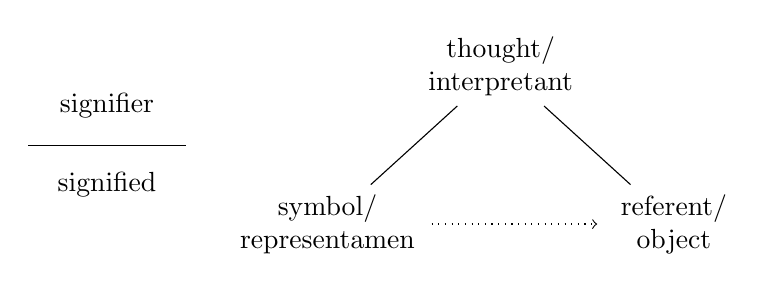
\begin{tikzpicture}
\begin{scope}[xshift=-50mm,yshift=10mm]
\node at (0,5mm) {signifier};
\node at (0,-5mm) {signified};
\draw (-1,0) to (1,0);
\end{scope}
\node[text width=24mm,align=center] at (-22mm,0) (symbol) {symbol/\\representamen};
\node[text width=17mm,align=center] at (22mm,0) (referent) {referent/ object};
\node[text width=20mm,align=center] at (0,2) (thought) {thought/ interpretant};
\draw (symbol) to (thought) (thought) to (referent);
\draw[dotted,->] (symbol) -> (referent);
\end{tikzpicture}
\caption{Dyadic and triadic models of a sign}
\label{fig:signmodels}
\end{figure}

The \term{arbitrarity} of the connection between signifier and signified, based
on social convention, is important to understand that there is no `natural' or
`true' relation between expression and content and that the relation cannot be
derived automatically.  Nevertheless the relation is not random. In addition to
fully arbitrary \Term{symbolic sign}s, Peirce distinguishes \Term{iconic sign}s
with some similarity between symbol and thought (for instance a metaphor or parts
of diagrams as described in section~\ref{sec:diagrams}), and
\Term{indexical sign}s that are directly connected to their thought (for
instance physical traces). This distinction can help at least to explain some
use of data, for instance brackets for grouping and annotation. The
impossibility of automatic derivation neither prevents interpretation of
unknown signs. According to \textcite[section 1.11]{Eco1984} signs are
interpreted by \Term{abduction}. Figure~\ref{fig:reasong} compares abduction
with other methods of logical reasoning: solid boxes indicate known
propositions and dotted boxes indicate tentative propositions produced in the
process of reasoning. Only \Term{deduction} can automatically
\term[inference]{infere} new results by application of formal \term{logic}: for
instance if all objects of type $A$ have some property $B$ (rule) and $a$ is of
type $A$ (case) then $a$ must also have property $B$ (result). Inductive
reasoning reconstructs the meaning of a sign through repeated experiences. If
objects are experienced to have property $B$ every time they are of type $A$,
one may conclude a general rule from these examples. Abduction, in contrast,
directly concludes a rule from a result. In the case of signs, the content is
concluded as as hypothesis from the expression.  For instance if $a$ has some
property $B$, one may presume some type $A$ that is responsible for having $B$.
The abductive diagnosis is often exemplified by detectives which work with
indications.\footnote{The name of William of Baskerville, Eco's main
protagonist in `The name of the Rose', is an allusion to the famous fictional
detective \Person[Sherlock]{Holmes}.} As such, the interpretation of signs is
always tentative and it carries the danger of fallacies: the form of abductive
reasoning is equal to the logical fallacy `post hoc ergo propter hoc' that
takes temporal sequence with casuality.

\begin{figure}
\centering
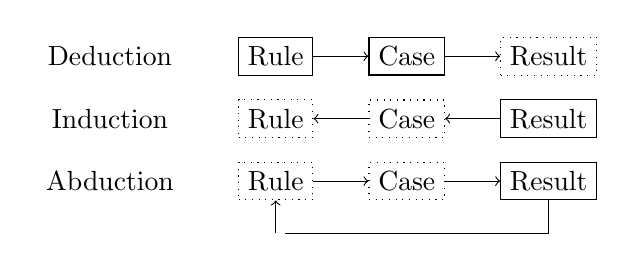
\begin{tikzpicture}
\matrix [column sep=7mm,row sep=3mm,dada/.style={draw,dotted}] {
 \node {Deduction}; & \node(m11)[draw]{Rule};   & \node(m21)[draw]{Case}; & \node(m31)[dada]{Result}; \\
 \node {Induction}; & \node(m12)[dada]{Rule}; & \node(m22)[dada]{Case}; & \node(m32)[draw]{Result}; \\
 \node {Abduction}; & \node(m13)[dada]{Rule}; & \node(m23)[dada]{Case}; & \node(m33)[draw]{Result}; \\
 & \node(m24){}; & \\
};
\draw[->] (m11) to (m21); \draw[->] (m21) to (m31);
\draw[->] (m22) to (m12); \draw[->] (m32) to (m22);
\draw[->] (m13) to (m23); \draw[->] (m23) to (m33);
\draw[->] (m33) |- (m24) -| (m13);
\end{tikzpicture}
\caption{Methods of reasoning, as illustrated by \textcite{Eco1984}}
\label{fig:reasong}
\end{figure}

\subsubsection{Signs are not isolated}

The third result from semiology consists of the fact that signs rarely occur
alone. Instead they are used in a system together with other signs. This system
as described by \person[Charles Sanders]{Peirce} is a language (`langue'), in
contrast to the actual use of a sign in communication (`parole'). The term
language should not be limited to \term[formal language]{formal languages} as
they are described in section~\ref{sec:formallanguages}.  Applied to data as
signs, digital objects do not occur alone, but they are collected and combined
with other digital objects. This collection and combination again is a method
of data structuring. Based on \person[Ferdinand]{e Saussure},
\textcite{Hjelmslev1953} identified syntagm and paradigm as two fundamental
relations by which elements of a language can be connected.

A \Term[syntagm]{syntagmatic} relation consists between elements which occur
together.  An example of syntagmatically connected data elements are \term{file
name}, \term{file type}, and \term{file extension}. Syntagm also provides
context in form of a structure in which elements can be embedded, but syntagm
is not limited to syntax and grammar. Similar elements that can be embedded in
same places are connected by \Term[paradigm]{paradigmatic} relations. Examples
of data elements connected by a paradigmatic relation are arrays and lists, and
the different \acro{RDF} nodes types which can all be used as object in an
\acro{RDF} triple (see table~\ref{tab:rdfvariants}). The final collection of
data patterns (chapter~\ref{ch:patterns}) also includes paradigmatic links
between patterns (as `alternative patterns') and syntagmatic links between
patterns (as `implied`, `specialized` and `related patterns`).

%\Term{paradigm} (from the Greek $\pi \alpha \rho \acute{\alpha} \delta \epsilon \imath
%\gamma \mu \alpha$ for `sample`, `example`, `pattern`) \ldots


\subsubsection{Further insights}

More insights from semiotics and linguistics may be possible if we take into
account the acts of communication which signs are used in. The usual
classification of communication studies includes aspects of \Term{syntax}
(relationships among signs, without reference to their meaning),
\Term{semantics} (relationships between signs and meanings), and
\Term{pragmatics} (relationships between signs and their use). Detailed models
of communication are given for instance by \textcite{Jakobson1963}, in the
theory of \Term{speech acts} \cite{Austin1962,Searle1969}, and in discourse
analysis \cite{Foucault1969}. For the following analysis, however, details of
communication are ignored because our focus is not the situation in which data
is used but the way it is structured and described. Neither does this thesis
include the diachronous nature of data, that is the temporal context in which
it changes. The difference between synchronity and diachronity has also been
introduced by de Saussure, an introduction to this opposition with
application to information as sign is given by \textcite{Raber2003}.

In summary, semiotics provides fruitfull insights to the nature of data, even
with limitation to immutable properties. Taking into account the full nature 
of signs, there are many issues left for further research in data semiotics.



\section{Patterns and pattern languages}
\label{sec:patterntheory}

\begin{quotation}%
Design and programming are human activities; forget that and all is lost.
\\\quotationsource \Person[Bjarne]{Stroustrup} (\citeyear{Stroustrup1997})
%  The C++ Programming Language. pp. 693.
\end{quotation}

\noindent The novel approach of this thesis is to use \Term[pattern]{patterns}
for data description, independent from particular structuring methods and
technologies. This section will first introduce the notion of patterns, then
summarize existing works that deal with patterns in data structuring and
finally give an example.

Patterns as systematic tools for describing good design practice were first
introduced by \Person[Christopher]{Alexander}, \Person[Sarah]{Ishikawa}, and
\Person[Murray]{Silverstein} \citeyear{Alexander1977}. They identified 253
existing architectural patterns from entire regions and cities to buildings,
rooms, and furniture. In Alexander's original definition \citeyear[p.
x]{Alexander1977} ``each pattern describes a problem which occurs over and over
again in our environment, and then describes the core of the solution to that
problem, in such a way that you can use this solution a million times over,
without ever doing it the same way twice.'' Patterns can be found by observing
current practice and then looking for commonalities in solutions to a problem.
In contrast to simple rules or best practice guidelines, a pattern, however,
does not solve the problem by providing a particular solution, but by showing
benefits and consequences. Each pattern provides a solution and each solution
has some tradeoffs. The pattern description guides designers in their decisions
of particular solutions for particular applications. Each pattern is given a
name, which can be used to refer to one pattern from another. The full
potential of patterns unfolds if a set of patterns is collected and combined in
a \Term{pattern language}. In Alexander's words ``a pattern language is a
network of patterns that call upon one another. Patterns help us remember
insights and knowledge about design and can be used in combination to create
solutions.`` A pattern language for writing patterns was presented by
\textcite{Meszaros1997}.

The pattern language approach with its application in architecture has been
adopted in other fields of engineering, especially in \term{software
engineering} \cite{Beck1987}.  \Person[Erich]{Gamma}, \Person[Richard]{Helm},
\Person[Ralph]{Johnson}, and \Person[John]{Vlissides} (the so-called `gang of
four') published an influental book on \Term{design patterns} in object
oriented programming \cite{Gamma1994}.  In 1995 \Person[Ward]{Cunningham}
created the Portland Pattern Repository \cite{Cunnigham1995}, accompanied by
WikiWikiWeb, which was the world's first \term{wiki}.\footnote{The Portland
Pattern Repository and WikiWikiWeb are still active at \url{http://c2.com/}.}

Although these design patterns are used for the creation of computer programs,
they do not reflect problems and solutions of data structuring as analyzed in
this thesis. Design patterns refer to dynamic processes, while digital documents
are static.  General patterns in description and structuring of data must also
be separated from \Term{pattern recognition}, as practiced in \term{data
mining} and other statistical methods of \term{machine learning}. These
quantitative methods can only recognize structures within the boundaries of a
fixed method of data description (for instance statistical patterns in lists of
numbers without questioning the nature of numbers and lists). A general
limitation of existing approaches is the focus to one specific formalization
method. This practical limitation blocks the view to more general data
patterns, independent from a particular encoding, and it conceals blind spots
and weaknesses of a chosen formalism. Some works about patterns in particular
data description languages have been mentioned in
section~\ref{sec:relatedworks}.

\subsectionexample{One data element, many patterns}

The following example shall illustrate the application of patterns in data
description. The patterns mentioned here anticipate members of the final
pattern language summarized in chapter~\ref{ch:patterns}. A more complex
example is given in appendix~\ref{appendixD}.

Given the following sequence of twelve bytes: 

\begin{center}
\verb|44 75 62 6c 69 6e 2c 20 4f 68 69 6f|\\
\end{center}

\noindent How can this particular piece of data be structured and described? To
start with, we need at least some context or indication. Let's assume each byte
corresponds to one character. This kind of correspondence can be summarizes as
\pattern{encoding} pattern. Given ASCII or Unicode encoding, the sequence is:

\begin{center}
\verb|Dublin, Ohio|
\end{center}

\noindent Several patterns provide obvious solutions to further description:

\begin{itemize}

	\item The data may be a list of two elements, \texttt{Dublin} 
		  and \texttt{Ohio}	(\pattern{sequence} pattern).

	\item It may consist of two elements as part of an unsorted collection
		  (\pattern{container} pattern), so
	      \texttt{Ohio, Dublin} should be equal to \texttt{Dublin, Ohio}.

	\item It may just refer to the name ``Dublin, Ohio'' without any 
		  relevant structure (\pattern{label} pattern).

    \item It may consist of two words, one of which (\texttt{Ohio}) being 
		  used as qualifier for the other (\texttt{Dublin}).

\end{itemize}

\noindent Given the last interpretation, a \emph{qualifier} may be a pattern in
its own right or it may be an example of a more general \pattern{flag} pattern
to indicate the interpretation of one element (\texttt{Dublin}) by another
(\texttt{Ohio}).

One can further deconstruct the structure of a data element to parts, a typical
process of description (\pattern{schema} pattern):

\begin{center}
$\underbrace{\texttt{Dublin}}_{1}%
\underbrace{\texttt{, }}_{2}%
\underbrace{\texttt{Ohio}}_{3}$
\end{center}

\noindent The third part is attached as additional element to the first 
(\pattern{dependence} pattern), and it may unambiguously refer into a registry of
allowed qualification values (\pattern{identifier} pattern). The second part
acts as connection or delimiter (\pattern{separator} pattern). Even its two
bytes (\texttt{, }) can have structure: the whitespace character is often
used as filling without significance (\pattern{garbage} pattern).

In summary one can identify several typical structuring methods in the twelve
bytes given above. The interpretation, however, does not need to be right ---
depending on context the sequence could mean virtually anything --- but
patterns help to reveal interpretations that were most likely intended when
creating the data.




